\documentclass{article}
\usepackage[utf8]{inputenc}

\title{Final Exam Problem 1 }
\author{Yuancheng Xu}
\date{Dec 17, 2020}

% Optional math commands from https://github.com/goodfeli/dlbook_notation.
%%%%% NEW MATH DEFINITIONS %%%%%

\usepackage{amsmath,amsfonts,bm}

% Mark sections of captions for referring to divisions of figures
\newcommand{\figleft}{{\em (Left)}}
\newcommand{\figcenter}{{\em (Center)}}
\newcommand{\figright}{{\em (Right)}}
\newcommand{\figtop}{{\em (Top)}}
\newcommand{\figbottom}{{\em (Bottom)}}
\newcommand{\captiona}{{\em (a)}}
\newcommand{\captionb}{{\em (b)}}
\newcommand{\captionc}{{\em (c)}}
\newcommand{\captiond}{{\em (d)}}

% Highlight a newly defined term
\newcommand{\newterm}[1]{{\bf #1}}


% Figure reference, lower-case.
\def\figref#1{figure~\ref{#1}}
% Figure reference, capital. For start of sentence
\def\Figref#1{Figure~\ref{#1}}
\def\twofigref#1#2{figures \ref{#1} and \ref{#2}}
\def\quadfigref#1#2#3#4{figures \ref{#1}, \ref{#2}, \ref{#3} and \ref{#4}}
% Section reference, lower-case.
\def\secref#1{section~\ref{#1}}
% Section reference, capital.
\def\Secref#1{Section~\ref{#1}}
% Reference to two sections.
\def\twosecrefs#1#2{sections \ref{#1} and \ref{#2}}
% Reference to three sections.
\def\secrefs#1#2#3{sections \ref{#1}, \ref{#2} and \ref{#3}}
% Reference to an equation, lower-case.
\def\eqref#1{equation~\ref{#1}}
% Reference to an equation, upper case
\def\Eqref#1{Equation~\ref{#1}}
% A raw reference to an equation---avoid using if possible
\def\plaineqref#1{\ref{#1}}
% Reference to a chapter, lower-case.
\def\chapref#1{chapter~\ref{#1}}
% Reference to an equation, upper case.
\def\Chapref#1{Chapter~\ref{#1}}
% Reference to a range of chapters
\def\rangechapref#1#2{chapters\ref{#1}--\ref{#2}}
% Reference to an algorithm, lower-case.
\def\algref#1{algorithm~\ref{#1}}
% Reference to an algorithm, upper case.
\def\Algref#1{Algorithm~\ref{#1}}
\def\twoalgref#1#2{algorithms \ref{#1} and \ref{#2}}
\def\Twoalgref#1#2{Algorithms \ref{#1} and \ref{#2}}
% Reference to a part, lower case
\def\partref#1{part~\ref{#1}}
% Reference to a part, upper case
\def\Partref#1{Part~\ref{#1}}
\def\twopartref#1#2{parts \ref{#1} and \ref{#2}}

\def\ceil#1{\lceil #1 \rceil}
\def\floor#1{\lfloor #1 \rfloor}
\def\1{\bm{1}}
\newcommand{\train}{\mathcal{D}}
\newcommand{\valid}{\mathcal{D_{\mathrm{valid}}}}
\newcommand{\test}{\mathcal{D_{\mathrm{test}}}}

\def\eps{{\epsilon}}


% Random variables
\def\reta{{\textnormal{$\eta$}}}
\def\ra{{\textnormal{a}}}
\def\rb{{\textnormal{b}}}
\def\rc{{\textnormal{c}}}
\def\rd{{\textnormal{d}}}
\def\re{{\textnormal{e}}}
\def\rf{{\textnormal{f}}}
\def\rg{{\textnormal{g}}}
\def\rh{{\textnormal{h}}}
\def\ri{{\textnormal{i}}}
\def\rj{{\textnormal{j}}}
\def\rk{{\textnormal{k}}}
\def\rl{{\textnormal{l}}}
% rm is already a command, just don't name any random variables m
\def\rn{{\textnormal{n}}}
\def\ro{{\textnormal{o}}}
\def\rp{{\textnormal{p}}}
\def\rq{{\textnormal{q}}}
\def\rr{{\textnormal{r}}}
\def\rs{{\textnormal{s}}}
\def\rt{{\textnormal{t}}}
\def\ru{{\textnormal{u}}}
\def\rv{{\textnormal{v}}}
\def\rw{{\textnormal{w}}}
\def\rx{{\textnormal{x}}}
\def\ry{{\textnormal{y}}}
\def\rz{{\textnormal{z}}}

% Random vectors
\def\rvepsilon{{\mathbf{\epsilon}}}
\def\rvtheta{{\mathbf{\theta}}}
\def\rva{{\mathbf{a}}}
\def\rvb{{\mathbf{b}}}
\def\rvc{{\mathbf{c}}}
\def\rvd{{\mathbf{d}}}
\def\rve{{\mathbf{e}}}
\def\rvf{{\mathbf{f}}}
\def\rvg{{\mathbf{g}}}
\def\rvh{{\mathbf{h}}}
\def\rvu{{\mathbf{i}}}
\def\rvj{{\mathbf{j}}}
\def\rvk{{\mathbf{k}}}
\def\rvl{{\mathbf{l}}}
\def\rvm{{\mathbf{m}}}
\def\rvn{{\mathbf{n}}}
\def\rvo{{\mathbf{o}}}
\def\rvp{{\mathbf{p}}}
\def\rvq{{\mathbf{q}}}
\def\rvr{{\mathbf{r}}}
\def\rvs{{\mathbf{s}}}
\def\rvt{{\mathbf{t}}}
\def\rvu{{\mathbf{u}}}
\def\rvv{{\mathbf{v}}}
\def\rvw{{\mathbf{w}}}
\def\rvx{{\mathbf{x}}}
\def\rvy{{\mathbf{y}}}
\def\rvz{{\mathbf{z}}}

% Elements of random vectors
\def\erva{{\textnormal{a}}}
\def\ervb{{\textnormal{b}}}
\def\ervc{{\textnormal{c}}}
\def\ervd{{\textnormal{d}}}
\def\erve{{\textnormal{e}}}
\def\ervf{{\textnormal{f}}}
\def\ervg{{\textnormal{g}}}
\def\ervh{{\textnormal{h}}}
\def\ervi{{\textnormal{i}}}
\def\ervj{{\textnormal{j}}}
\def\ervk{{\textnormal{k}}}
\def\ervl{{\textnormal{l}}}
\def\ervm{{\textnormal{m}}}
\def\ervn{{\textnormal{n}}}
\def\ervo{{\textnormal{o}}}
\def\ervp{{\textnormal{p}}}
\def\ervq{{\textnormal{q}}}
\def\ervr{{\textnormal{r}}}
\def\ervs{{\textnormal{s}}}
\def\ervt{{\textnormal{t}}}
\def\ervu{{\textnormal{u}}}
\def\ervv{{\textnormal{v}}}
\def\ervw{{\textnormal{w}}}
\def\ervx{{\textnormal{x}}}
\def\ervy{{\textnormal{y}}}
\def\ervz{{\textnormal{z}}}

% Random matrices
\def\rmA{{\mathbf{A}}}
\def\rmB{{\mathbf{B}}}
\def\rmC{{\mathbf{C}}}
\def\rmD{{\mathbf{D}}}
\def\rmE{{\mathbf{E}}}
\def\rmF{{\mathbf{F}}}
\def\rmG{{\mathbf{G}}}
\def\rmH{{\mathbf{H}}}
\def\rmI{{\mathbf{I}}}
\def\rmJ{{\mathbf{J}}}
\def\rmK{{\mathbf{K}}}
\def\rmL{{\mathbf{L}}}
\def\rmM{{\mathbf{M}}}
\def\rmN{{\mathbf{N}}}
\def\rmO{{\mathbf{O}}}
\def\rmP{{\mathbf{P}}}
\def\rmQ{{\mathbf{Q}}}
\def\rmR{{\mathbf{R}}}
\def\rmS{{\mathbf{S}}}
\def\rmT{{\mathbf{T}}}
\def\rmU{{\mathbf{U}}}
\def\rmV{{\mathbf{V}}}
\def\rmW{{\mathbf{W}}}
\def\rmX{{\mathbf{X}}}
\def\rmY{{\mathbf{Y}}}
\def\rmZ{{\mathbf{Z}}}

% Elements of random matrices
\def\ermA{{\textnormal{A}}}
\def\ermB{{\textnormal{B}}}
\def\ermC{{\textnormal{C}}}
\def\ermD{{\textnormal{D}}}
\def\ermE{{\textnormal{E}}}
\def\ermF{{\textnormal{F}}}
\def\ermG{{\textnormal{G}}}
\def\ermH{{\textnormal{H}}}
\def\ermI{{\textnormal{I}}}
\def\ermJ{{\textnormal{J}}}
\def\ermK{{\textnormal{K}}}
\def\ermL{{\textnormal{L}}}
\def\ermM{{\textnormal{M}}}
\def\ermN{{\textnormal{N}}}
\def\ermO{{\textnormal{O}}}
\def\ermP{{\textnormal{P}}}
\def\ermQ{{\textnormal{Q}}}
\def\ermR{{\textnormal{R}}}
\def\ermS{{\textnormal{S}}}
\def\ermT{{\textnormal{T}}}
\def\ermU{{\textnormal{U}}}
\def\ermV{{\textnormal{V}}}
\def\ermW{{\textnormal{W}}}
\def\ermX{{\textnormal{X}}}
\def\ermY{{\textnormal{Y}}}
\def\ermZ{{\textnormal{Z}}}

% Vectors
\def\vzero{{\bm{0}}}
\def\vone{{\bm{1}}}
\def\vmu{{\bm{\mu}}}
\def\vtheta{{\bm{\theta}}}
\def\va{{\bm{a}}}
\def\vb{{\bm{b}}}
\def\vc{{\bm{c}}}
\def\vd{{\bm{d}}}
\def\ve{{\bm{e}}}
\def\vf{{\bm{f}}}
\def\vg{{\bm{g}}}
\def\vh{{\bm{h}}}
\def\vi{{\bm{i}}}
\def\vj{{\bm{j}}}
\def\vk{{\bm{k}}}
\def\vl{{\bm{l}}}
\def\vm{{\bm{m}}}
\def\vn{{\bm{n}}}
\def\vo{{\bm{o}}}
\def\vp{{\bm{p}}}
\def\vq{{\bm{q}}}
\def\vr{{\bm{r}}}
\def\vs{{\bm{s}}}
\def\vt{{\bm{t}}}
\def\vu{{\bm{u}}}
\def\vv{{\bm{v}}}
\def\vw{{\bm{w}}}
\def\vx{{\bm{x}}}
\def\vy{{\bm{y}}}
\def\vz{{\bm{z}}}

% Elements of vectors
\def\evalpha{{\alpha}}
\def\evbeta{{\beta}}
\def\evepsilon{{\epsilon}}
\def\evlambda{{\lambda}}
\def\evomega{{\omega}}
\def\evmu{{\mu}}
\def\evpsi{{\psi}}
\def\evsigma{{\sigma}}
\def\evtheta{{\theta}}
\def\eva{{a}}
\def\evb{{b}}
\def\evc{{c}}
\def\evd{{d}}
\def\eve{{e}}
\def\evf{{f}}
\def\evg{{g}}
\def\evh{{h}}
\def\evi{{i}}
\def\evj{{j}}
\def\evk{{k}}
\def\evl{{l}}
\def\evm{{m}}
\def\evn{{n}}
\def\evo{{o}}
\def\evp{{p}}
\def\evq{{q}}
\def\evr{{r}}
\def\evs{{s}}
\def\evt{{t}}
\def\evu{{u}}
\def\evv{{v}}
\def\evw{{w}}
\def\evx{{x}}
\def\evy{{y}}
\def\evz{{z}}

% Matrix
\def\mA{{\bm{A}}}
\def\mB{{\bm{B}}}
\def\mC{{\bm{C}}}
\def\mD{{\bm{D}}}
\def\mE{{\bm{E}}}
\def\mF{{\bm{F}}}
\def\mG{{\bm{G}}}
\def\mH{{\bm{H}}}
\def\mI{{\bm{I}}}
\def\mJ{{\bm{J}}}
\def\mK{{\bm{K}}}
\def\mL{{\bm{L}}}
\def\mM{{\bm{M}}}
\def\mN{{\bm{N}}}
\def\mO{{\bm{O}}}
\def\mP{{\bm{P}}}
\def\mQ{{\bm{Q}}}
\def\mR{{\bm{R}}}
\def\mS{{\bm{S}}}
\def\mT{{\bm{T}}}
\def\mU{{\bm{U}}}
\def\mV{{\bm{V}}}
\def\mW{{\bm{W}}}
\def\mX{{\bm{X}}}
\def\mY{{\bm{Y}}}
\def\mZ{{\bm{Z}}}
\def\mBeta{{\bm{\beta}}}
\def\mPhi{{\bm{\Phi}}}
\def\mLambda{{\bm{\Lambda}}}
\def\mSigma{{\bm{\Sigma}}}

% Tensor
\DeclareMathAlphabet{\mathsfit}{\encodingdefault}{\sfdefault}{m}{sl}
\SetMathAlphabet{\mathsfit}{bold}{\encodingdefault}{\sfdefault}{bx}{n}
\newcommand{\tens}[1]{\bm{\mathsfit{#1}}}
\def\tA{{\tens{A}}}
\def\tB{{\tens{B}}}
\def\tC{{\tens{C}}}
\def\tD{{\tens{D}}}
\def\tE{{\tens{E}}}
\def\tF{{\tens{F}}}
\def\tG{{\tens{G}}}
\def\tH{{\tens{H}}}
\def\tI{{\tens{I}}}
\def\tJ{{\tens{J}}}
\def\tK{{\tens{K}}}
\def\tL{{\tens{L}}}
\def\tM{{\tens{M}}}
\def\tN{{\tens{N}}}
\def\tO{{\tens{O}}}
\def\tP{{\tens{P}}}
\def\tQ{{\tens{Q}}}
\def\tR{{\tens{R}}}
\def\tS{{\tens{S}}}
\def\tT{{\tens{T}}}
\def\tU{{\tens{U}}}
\def\tV{{\tens{V}}}
\def\tW{{\tens{W}}}
\def\tX{{\tens{X}}}
\def\tY{{\tens{Y}}}
\def\tZ{{\tens{Z}}}


% Graph
\def\gA{{\mathcal{A}}}
\def\gB{{\mathcal{B}}}
\def\gC{{\mathcal{C}}}
\def\gD{{\mathcal{D}}}
\def\gE{{\mathcal{E}}}
\def\gF{{\mathcal{F}}}
\def\gG{{\mathcal{G}}}
\def\gH{{\mathcal{H}}}
\def\gI{{\mathcal{I}}}
\def\gJ{{\mathcal{J}}}
\def\gK{{\mathcal{K}}}
\def\gL{{\mathcal{L}}}
\def\gM{{\mathcal{M}}}
\def\gN{{\mathcal{N}}}
\def\gO{{\mathcal{O}}}
\def\gP{{\mathcal{P}}}
\def\gQ{{\mathcal{Q}}}
\def\gR{{\mathcal{R}}}
\def\gS{{\mathcal{S}}}
\def\gT{{\mathcal{T}}}
\def\gU{{\mathcal{U}}}
\def\gV{{\mathcal{V}}}
\def\gW{{\mathcal{W}}}
\def\gX{{\mathcal{X}}}
\def\gY{{\mathcal{Y}}}
\def\gZ{{\mathcal{Z}}}

% Sets
\def\sA{{\mathbb{A}}}
\def\sB{{\mathbb{B}}}
\def\sC{{\mathbb{C}}}
\def\sD{{\mathbb{D}}}
% Don't use a set called E, because this would be the same as our symbol
% for expectation.
\def\sF{{\mathbb{F}}}
\def\sG{{\mathbb{G}}}
\def\sH{{\mathbb{H}}}
\def\sI{{\mathbb{I}}}
\def\sJ{{\mathbb{J}}}
\def\sK{{\mathbb{K}}}
\def\sL{{\mathbb{L}}}
\def\sM{{\mathbb{M}}}
\def\sN{{\mathbb{N}}}
\def\sO{{\mathbb{O}}}
\def\sP{{\mathbb{P}}}
\def\sQ{{\mathbb{Q}}}
\def\sR{{\mathbb{R}}}
\def\sS{{\mathbb{S}}}
\def\sT{{\mathbb{T}}}
\def\sU{{\mathbb{U}}}
\def\sV{{\mathbb{V}}}
\def\sW{{\mathbb{W}}}
\def\sX{{\mathbb{X}}}
\def\sY{{\mathbb{Y}}}
\def\sZ{{\mathbb{Z}}}

% Entries of a matrix
\def\emLambda{{\Lambda}}
\def\emA{{A}}
\def\emB{{B}}
\def\emC{{C}}
\def\emD{{D}}
\def\emE{{E}}
\def\emF{{F}}
\def\emG{{G}}
\def\emH{{H}}
\def\emI{{I}}
\def\emJ{{J}}
\def\emK{{K}}
\def\emL{{L}}
\def\emM{{M}}
\def\emN{{N}}
\def\emO{{O}}
\def\emP{{P}}
\def\emQ{{Q}}
\def\emR{{R}}
\def\emS{{S}}
\def\emT{{T}}
\def\emU{{U}}
\def\emV{{V}}
\def\emW{{W}}
\def\emX{{X}}
\def\emY{{Y}}
\def\emZ{{Z}}
\def\emSigma{{\Sigma}}

% entries of a tensor
% Same font as tensor, without \bm wrapper
\newcommand{\etens}[1]{\mathsfit{#1}}
\def\etLambda{{\etens{\Lambda}}}
\def\etA{{\etens{A}}}
\def\etB{{\etens{B}}}
\def\etC{{\etens{C}}}
\def\etD{{\etens{D}}}
\def\etE{{\etens{E}}}
\def\etF{{\etens{F}}}
\def\etG{{\etens{G}}}
\def\etH{{\etens{H}}}
\def\etI{{\etens{I}}}
\def\etJ{{\etens{J}}}
\def\etK{{\etens{K}}}
\def\etL{{\etens{L}}}
\def\etM{{\etens{M}}}
\def\etN{{\etens{N}}}
\def\etO{{\etens{O}}}
\def\etP{{\etens{P}}}
\def\etQ{{\etens{Q}}}
\def\etR{{\etens{R}}}
\def\etS{{\etens{S}}}
\def\etT{{\etens{T}}}
\def\etU{{\etens{U}}}
\def\etV{{\etens{V}}}
\def\etW{{\etens{W}}}
\def\etX{{\etens{X}}}
\def\etY{{\etens{Y}}}
\def\etZ{{\etens{Z}}}

% The true underlying data generating distribution
\newcommand{\pdata}{p_{\rm{data}}}
% The empirical distribution defined by the training set
\newcommand{\ptrain}{\hat{p}_{\rm{data}}}
\newcommand{\Ptrain}{\hat{P}_{\rm{data}}}
% The model distribution
\newcommand{\pmodel}{p_{\rm{model}}}
\newcommand{\Pmodel}{P_{\rm{model}}}
\newcommand{\ptildemodel}{\tilde{p}_{\rm{model}}}
% Stochastic autoencoder distributions
\newcommand{\pencode}{p_{\rm{encoder}}}
\newcommand{\pdecode}{p_{\rm{decoder}}}
\newcommand{\precons}{p_{\rm{reconstruct}}}

\newcommand{\laplace}{\mathrm{Laplace}} % Laplace distribution

\newcommand{\E}{\mathbb{E}}
\newcommand{\Ls}{\mathcal{L}}
\newcommand{\R}{\mathbb{R}}
\newcommand{\emp}{\tilde{p}}
\newcommand{\lr}{\alpha}
\newcommand{\reg}{\lambda}
\newcommand{\rect}{\mathrm{rectifier}}
\newcommand{\softmax}{\mathrm{softmax}}
\newcommand{\sigmoid}{\sigma}
\newcommand{\softplus}{\zeta}
\newcommand{\KL}{D_{\mathrm{KL}}}
\newcommand{\Var}{\mathrm{Var}}
\newcommand{\standarderror}{\mathrm{SE}}
\newcommand{\Cov}{\mathrm{Cov}}
% Wolfram Mathworld says $L^2$ is for function spaces and $\ell^2$ is for vectors
% But then they seem to use $L^2$ for vectors throughout the site, and so does
% wikipedia.
\newcommand{\normlzero}{L^0}
\newcommand{\normlone}{L^1}
\newcommand{\normltwo}{L^2}
\newcommand{\normlp}{L^p}
\newcommand{\normmax}{L^\infty}

\newcommand{\parents}{Pa} % See usage in notation.tex. Chosen to match Daphne's book.

\DeclareMathOperator*{\argmax}{arg\,max}
\DeclareMathOperator*{\argmin}{arg\,min}

\DeclareMathOperator{\sign}{sign}
\DeclareMathOperator{\Tr}{Tr}
\let\ab\allowbreak


\usepackage{natbib}
\usepackage{amsmath}
\usepackage{bm}
\usepackage{multirow}
\usepackage{amssymb}
\usepackage{hyperref}
\usepackage{url}
\usepackage{enumerate}
\usepackage{bbm}
\usepackage{graphicx}
\usepackage{pdfpages}
\usepackage{amsthm}
% \usepackage{subfigure}

% \DeclareMathOperator{\Tr}{Tr}

\newtheorem{theorem}{Theorem}[section]
\newtheorem{corollary}{Corollary}[theorem]
\newtheorem{lemma}[theorem]{Lemma}
\usepackage{subcaption}

\newcommand{\ReLU}{\text{ReLU}}

\begin{document}

\maketitle

%\noindent Code link:\\
%\url{https://github.com/Yuancheng-Xu/AMSC-808N/tree/master/HW6}\\

\section*{Q1: Analysis of the objective function}
Denote $ f_j(a,b) = [\ReLU(ax_j-b)-g(x_j)]^2 $ and $ y_j = g(x_j) $. Therefore 

\begin{equation} \label{eq: grad fj}
	\nabla f_j = 2(ax_j-b-y_j) \mathbbm{1}(ax_j-b>0) 
	\begin{bmatrix}
		x_j \\ -1
	\end{bmatrix}
\end{equation}

The stationary points of $ f $ corresponds to $ \sum_{j=0}^{5}\nabla f_j = 0 $. In this problem, $ 0 = x_0 < x_1 <...<x_5 $ and $ 0=y_0<y_1<...<y_5 = 1$. $ x_j $ is called activate if $ ax_j -b >0 $, and non-active otherwise.

Also, the Hessian $ Hf = \frac{1}{12}\sum_{j=0}^{5}Hf_j $, where $ Hf_j $ is given by

\begin{equation}
	Hf_j = 2 \mathbbm{1}(ax_j-b>0) 
	\begin{bmatrix}
		x_j^2 & -x_j \\ -x_j & 1
	\end{bmatrix}
\end{equation}

In this question, I would like to know the set of stationary points of $ f $. First, I decompose the parameter space into several components, each of which corresponds to 0 to 6 active points. This is visualize in Figure \ref{fig: space decomposition}. The stationary points are obtained as follows.
\begin{itemize}
	\item If $ (a,b) $ satisfies that none of $ x_j $ is active, it is obviously stationary and therefore the flat region (where all points are non-active) is stationary ($ f $ is constant in this region). Analytically, this flat region is given by $ \{b>0, b>x_5 a\} $ with $ x_5 = \frac{\pi}{2} $.
	
	\item  If only one of $ x_j $ is active (it can only be $ x_5 $ or $ x_0 $; note that since $ x_0 = 0 $ and $ y_0 = 0 $, $ b $ must be zero in order for the gradient to be zero, which corresponds to the boundary of the flat region and it is not interesting), let $ \nabla f_j = 0 $ (with $ j=5 $) in Equation \ref{eq: grad fj} and obtain $ b = ax_5 - y_5 $. Note that we need the constraint that $ a>0, b>ax_4 $ so that other points are not active. Analytically I obtain that the point $ p $ in Figure \ref{fig: space decomposition} is $ (\pi, \frac{\pi^2}{2}-1) $ and therefore the corresponding line of stationary points is $ \{b = ax_5 - y_5, a>\pi\} $.
	
	\item If n ($ n\geq 2 $) of $ x_j $ are active, the stationary point is either unique or does not exist. To see this, let $ \nabla f = 0 $ and obtain the following equation (least squares in one-dimension) 
	\begin{equation} \label{eq: linear}
	\begin{bmatrix}
		\sum x_j^2 & -\sum x_j \\ -\sum x_j & n
	\end{bmatrix} 
	\begin{bmatrix}
		a\\ b
	\end{bmatrix} =
	\begin{bmatrix}
		\sum x_j y_j\\ -\sum y_j
	\end{bmatrix} 
	\end{equation}

	where the sum is over the n activated $ j $. Note that this linear system has an unique solution when $ n \geq 2 $, with $ a = \frac{n\sum x_j y_j - (\sum x_j)(\sum y_j)}{n\sum x_j^2 - (\sum x_j)^2} $ and $ b = a \frac{\sum x_j}{n} - \frac{\sum y_j}{n} $. However, the solution must be inside the region where those n activated points are indeed activated, in order to be a stationary point of $ f $. For each component in Figure \ref{fig: space decomposition}, I solve the corresponding Equation \ref{eq: linear} and check whether it is in that component. It turns out that there is only one isolated stationary point $ x^{\ast} $, which is in the region where $ x_2, x_3, x_4 $ and $ x_5 $ are active. I can analytically obtain $ x^{*} $ by substituting $ \{x_j, y_j\}_{j=2}^{5} $  and $ n=4 $ into the above formula for $ a,b $. Since the exact formula is tedious, I obtain it numerically and $ x^{*} = (a^{*}, b^{*}) = (0.8613, 0.3735) $. The Hessian at $ x^{*} $ is positive definite and by comparing the $ f $ value with other stationary points, I conclude that it is the global minimizer with the global minimum $ f(x^{*}) = 3.6e-4 $. 
\end{itemize}

\begin{figure}[htp]
	\centering
	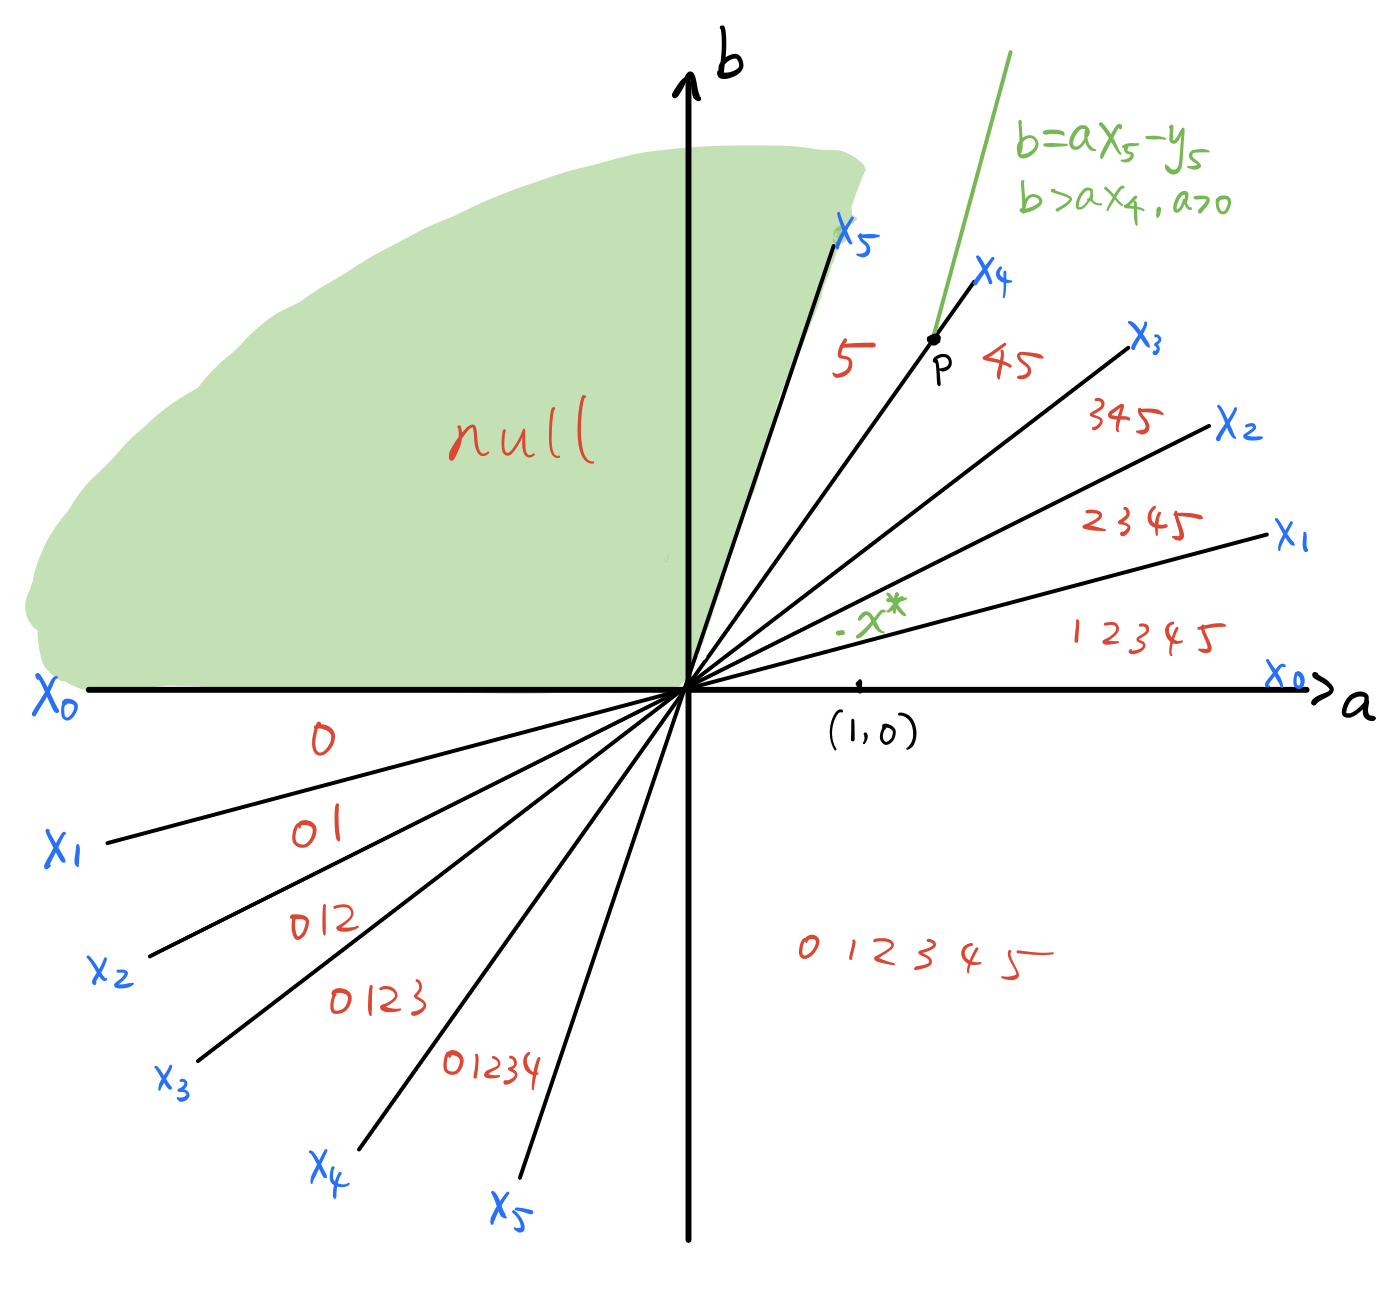
\includegraphics[width=.7\linewidth]{figs/SpaceDecompostion}
	\caption{Decomposition of the parameter space. In blue, the line with $ x_j $ means the line $ b = x_j a $. In red, the number indicates which points are activated, meaning that $ ax_j - b > 0 $. For example, '2345' means $ x_2,x_3,x_4,x_5 $ are activated. Finally, stationary points are in green. Note that they consist of a flat region, a line (with $ b=ax_5-y_5 $ where $ a>\pi $) and the global minimizer $ x^{*} $.}
	\label{fig: space decomposition}
\end{figure}

\section*{Q2: Gradient descent with constant stepsize}
First let us visualize the vector field of $ -\nabla f $ in Figure \ref{fig: vector field}.

\paragraph{Minimal stepsize $ \alpha^{*}$ that the iterates end up in the flat region} As we can see from Figure \ref{fig: vector field}, if the iterates were to enter the flat region, they would enter through the boundary  $ \{b>0, b=x_5 a\} $. On the outer part of the boundary, we have  $ -\nabla f = (\pi,-2)$, pointing outwards of the flat region. Therefore, in order to enter the flat region, the iterates should hit the boundary \textbf{at the first step}, which corresponds to the minimal stepsize $ \alpha^{*} $. If the actual step size is $ \alpha < \alpha^{*} $, it will bounce away from the boundary and never enter the flat region. Therefore, I obtain $ \alpha^{*} $ by letting the first step of the iterates (with direction $ -\nabla f  (1,0)$) hit $ \{b>0, b=x_5 a\} $ (that is, the point$ (a,b) = (1,0) - \alpha^{*}\nabla f  (1,0)  $ satisfies $  b=x_5 a\ $). Numerically, I obtain $ \alpha^{*} = 1.51 $, which corresponds to slightly overshooting the boundary at the first step).


\begin{figure} 
	\begin{subfigure}[b]{.5\linewidth}
		\centering\large 	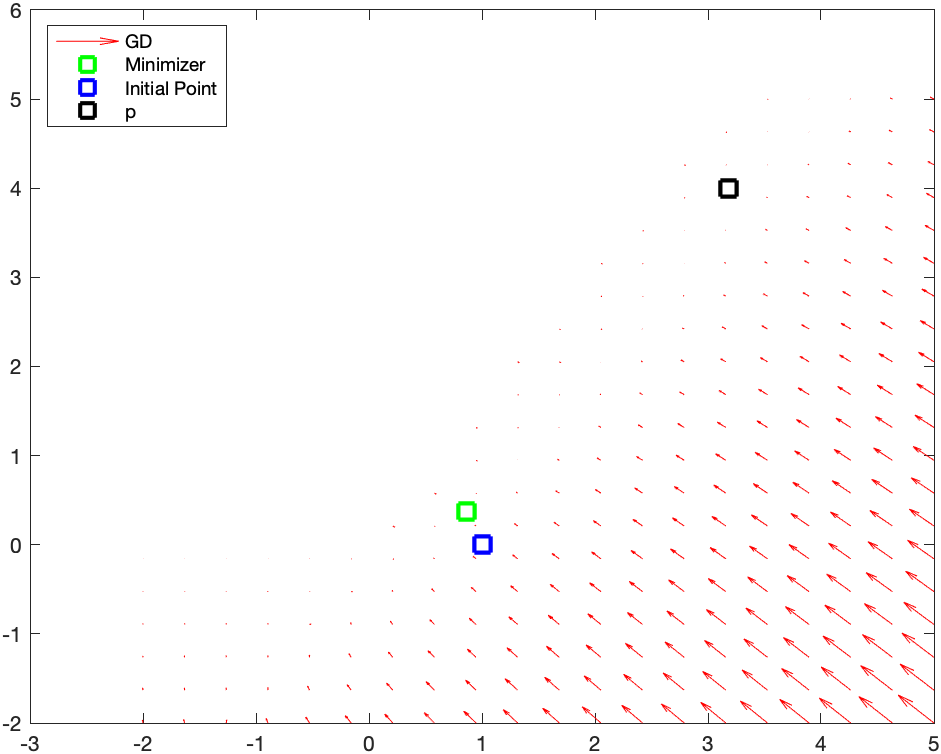
\includegraphics[width=\linewidth]{figs/vecfield_global}
		\caption{Global view.}\label{fig: vecfield_global}
	\end{subfigure}% 
	\begin{subfigure}[b]{.515\linewidth}
		\centering\large 	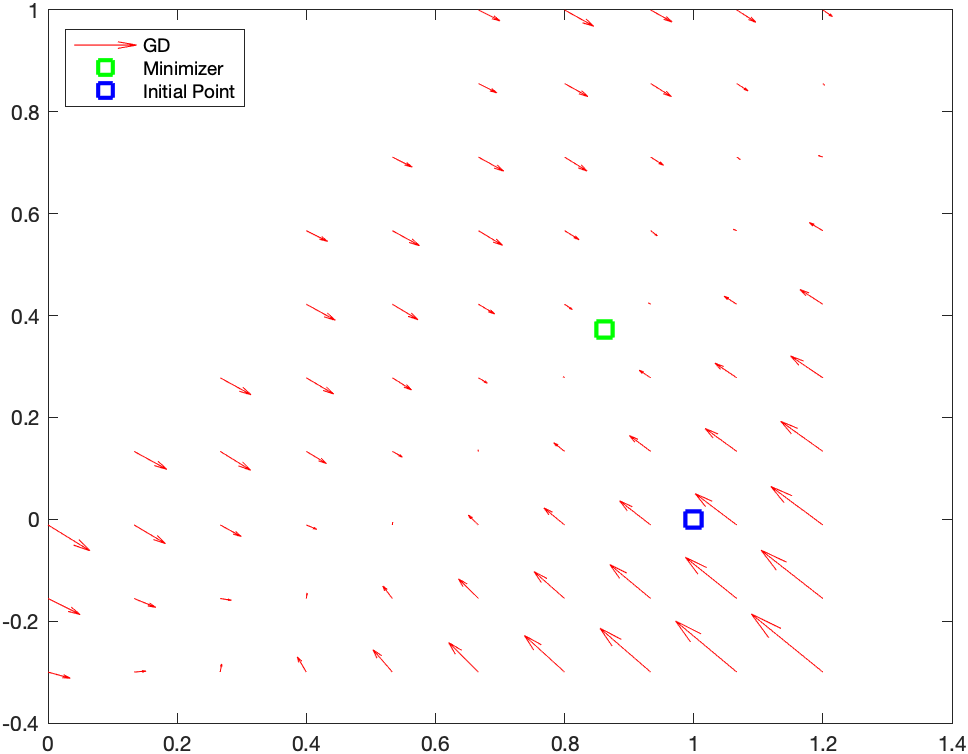
\includegraphics[width=\linewidth]{figs/vecfield_veryclose}
		\caption{Local view}\label{fig: vecfield_veryclose}
	\end{subfigure}
	\caption{The vector field around the minimizer and the initial point. At each point, the slope corresponds to the minus gradient of $ f $.}\label{fig: vector field}
\end{figure}

\paragraph{$ \alpha < \alpha^{*}$ does not necessarily results in convergence} In order to see this, I take $ \alpha = 0.99\alpha^{*} $ and the iterates are shown in Figure \ref{fig: Q2_99}, where they bounce between the two sides of the global minimizer without ever convergence to it. As a side-note, in MatLab I can actually see the iterates step-by-step by plotting each iterate in every iteration and setting breakpoints. To explain why $ \alpha = 0.99\alpha^{*} $ does not lead to convergence, note that in theory, the iterates need to enter a region where $ f $ is (strongly) convex in order to converge to $ x^{*} $. I find numerically that the smallest eigenvalue of the Hessian $ Hf $ at the global minimizer $ x^{*} $ is $ 0.03 $, which is small. This indicates that it is not so easy to enter that basin (which is indeed the case as we can see from Figure \ref{fig: Q2_99}) and explains why  $ \alpha = 0.99\alpha^{*} $ doesn't lead to convergence.

\begin{figure}[htp]
	\centering
	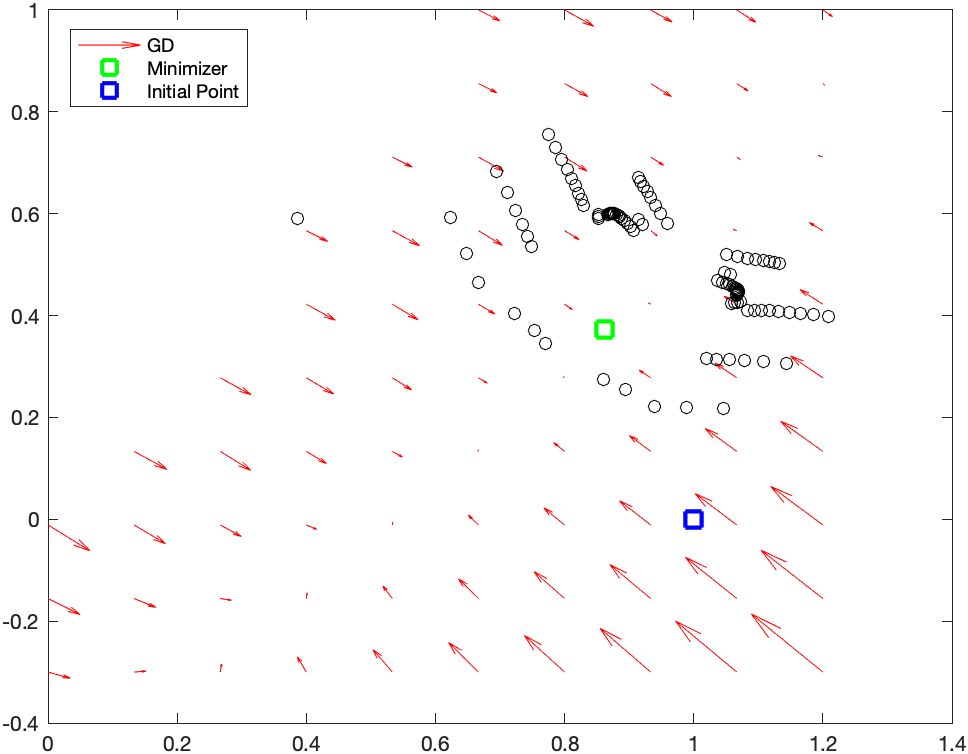
\includegraphics[width=.7\linewidth]{figs/Q2_99percent.png}
	\caption{Trajectories when $ \alpha = 0.99\alpha^{*} $. The first step misses the boundary of the flat region and the iterates bounce between the two sides of the global minimizer without ever convergence to it. }
	\label{fig: Q2_99}
\end{figure}

\paragraph{Finding the largest stepsize $ \alpha $ for convergence}  In order to find the stepsizes that result in convergence, I plot the trajectories using various $ \alpha $ in Figure \ref{fig: Q2_various}. Observe that $ \alpha_c = 1.31$ is the critical value for convergence (largest stepsize for convergence). When $ 0.7<\alpha < 1.31 $, the iterates will first hit the other side of the minimizer but eventually they converge. When $ \alpha < 0.7 $, the iterates never hit the other side and converge to the minimizer directly.

 

\begin{figure}[htp]
	
	\begin{subfigure}{.5\textwidth}
		\centering
		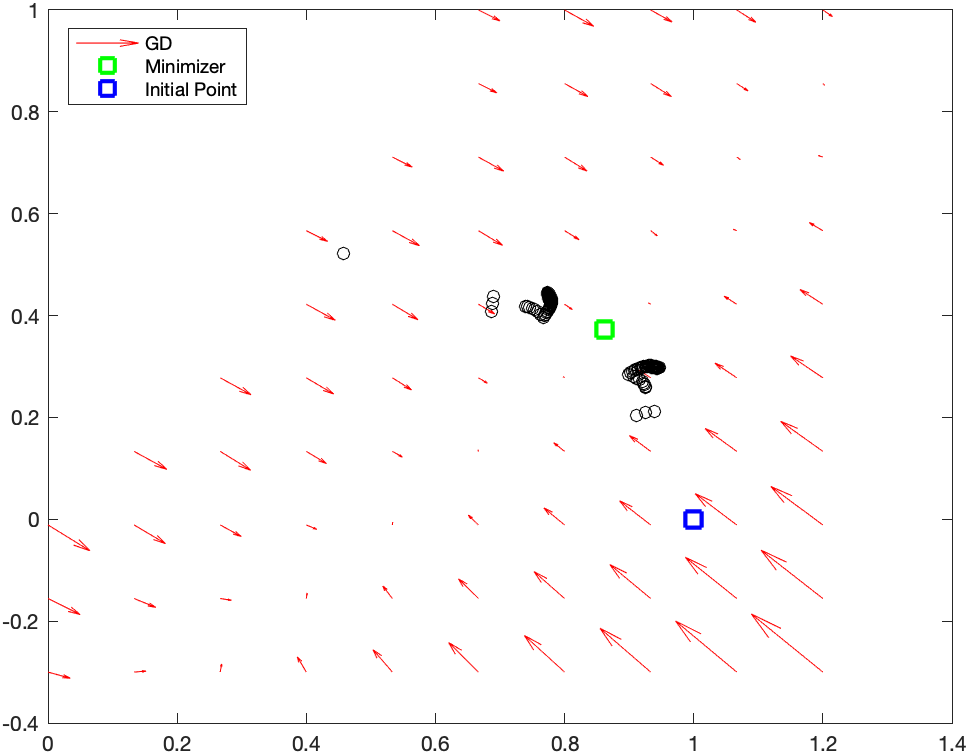
\includegraphics[width=.8\linewidth]{figs/Q2_132.png}
		\caption{$ \alpha = 1.32 $}
	\end{subfigure}
	\begin{subfigure}{.5\textwidth}
		\centering
		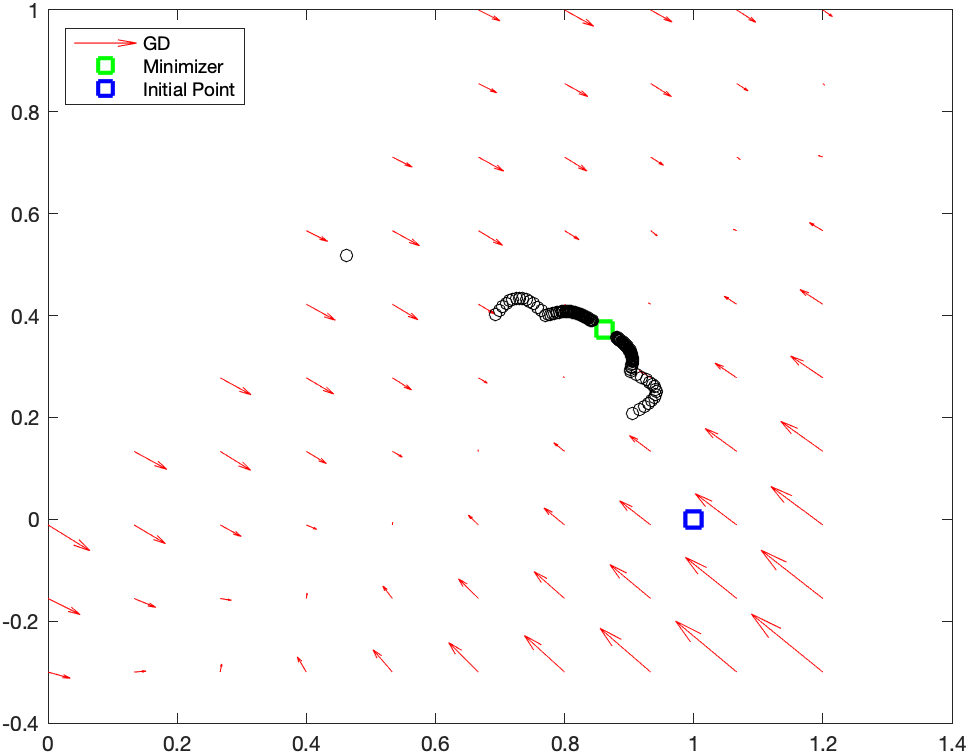
\includegraphics[width=.8\linewidth]{figs/Q2_131.png}
		\caption{$ \alpha = 1.31 $}
	\end{subfigure}
	\begin{subfigure}{.5\textwidth}
		\centering
		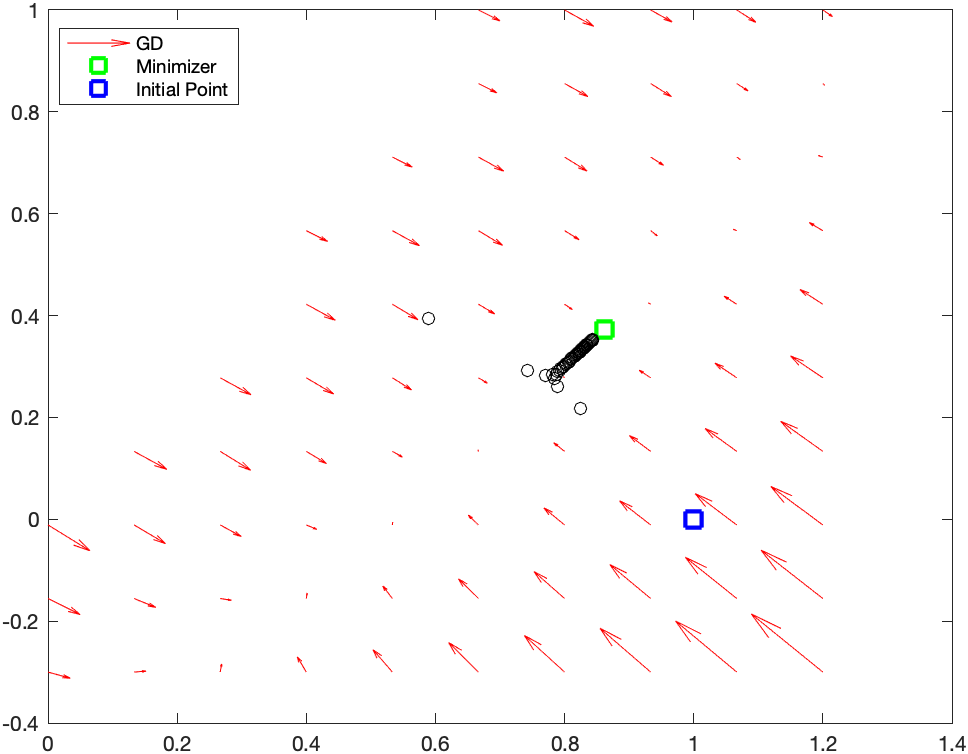
\includegraphics[width=.8\linewidth]{figs/Q2_100.png}
		\caption{$ \alpha = 1 $}
	\end{subfigure}
	\begin{subfigure}{.5\textwidth}
		\centering
		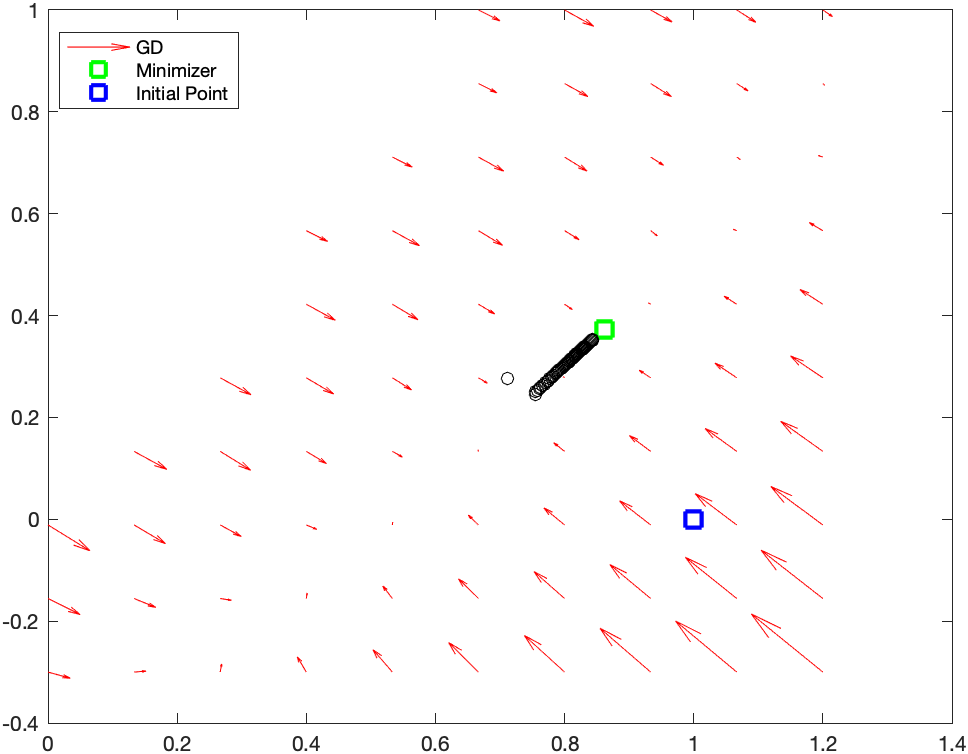
\includegraphics[width=.8\linewidth]{figs/Q2_70.png}
		\caption{$ \alpha = 0.7 $}
	\end{subfigure}
	\begin{subfigure}{.5\textwidth}
		\centering
		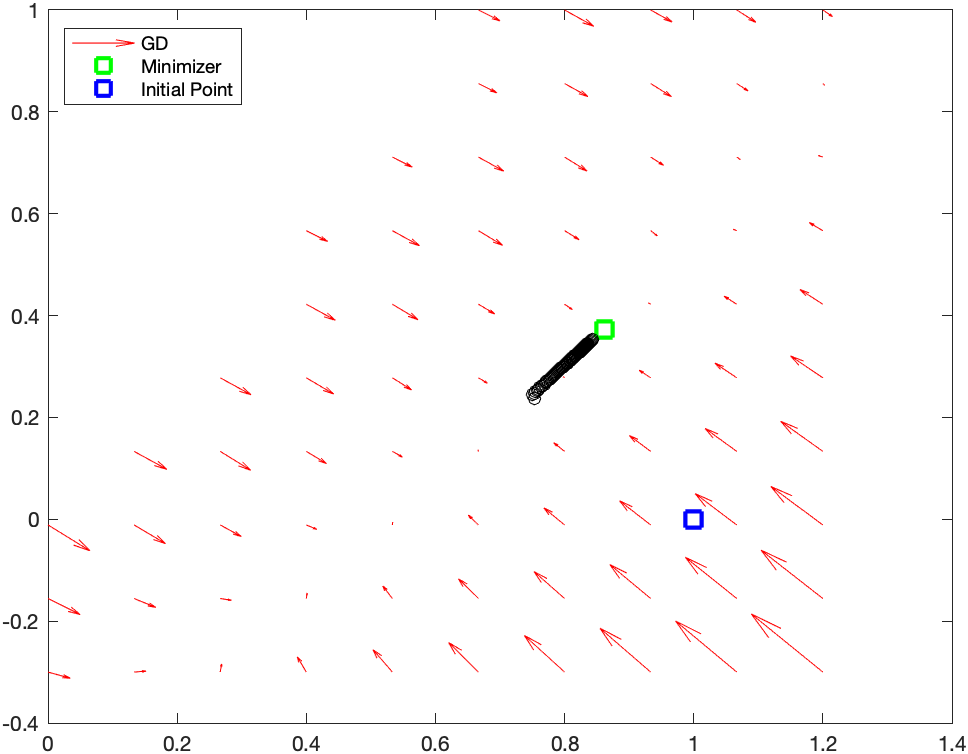
\includegraphics[width=.8\linewidth]{figs/Q2_60.png}
		\caption{$ \alpha = 0.6 $}
	\end{subfigure}
	\begin{subfigure}{.5\textwidth}
		\centering
		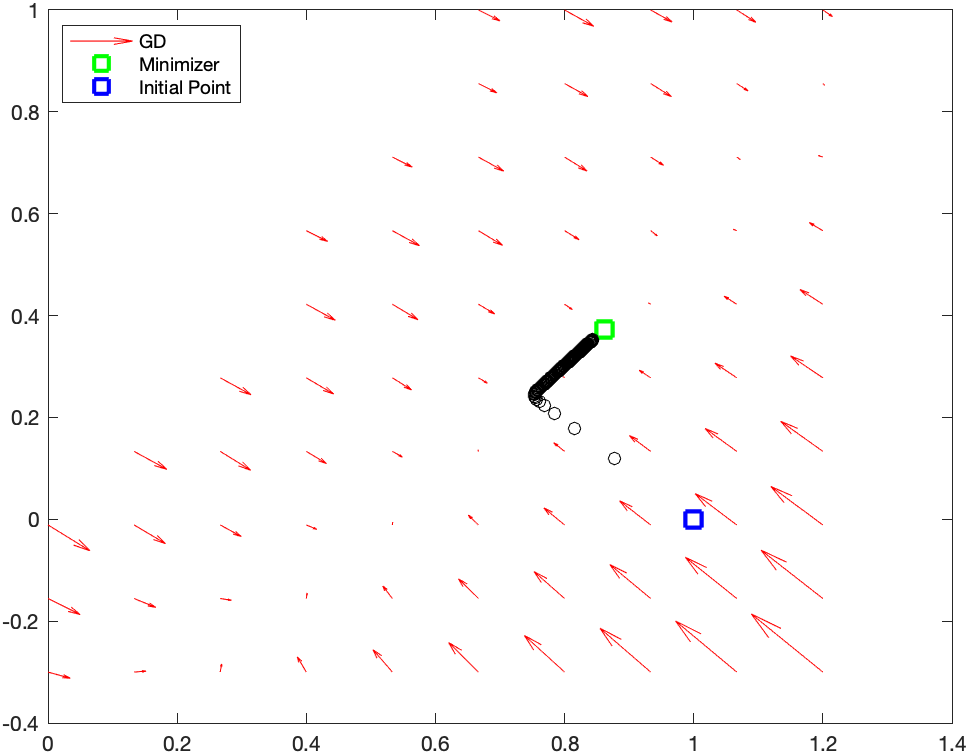
\includegraphics[width=.8\linewidth]{figs/Q2_30.png}
		\caption{$ \alpha = 0.3 $}
	\end{subfigure}
	
	\caption{Various convergence modes. Except for the first case ($ \alpha=1.32 $) which doesn't converge, several convergence modes (with or without oscillating) are shown.}
	\label{fig: Q2_various}
	
\end{figure}

\paragraph{But what is the best stepsize?} Since larger stepsize may lead to the oscillating behavior in this problem, and thus waste a lot of effort towards convergence, it is not necessary that larger stepsize will lead to faster convergence. Therefore, here I compare, for each $ \alpha $, the number of iterations needed for convergence (up to tolerance $ ||\nabla f||<1e-6 $). The result is shown in Figure \ref{fig:Q2_iteration_alpha}. Observe how the number of iterations first drop gently (due to the increase in stepsize) and then increase abruptly (due to the waste of effort in too much oscillating). The best stepsize is $ 1.2652 $. To understand the increase in the number of iterations, let us visualize the trajectories with $ \alpha = 1.2652 $ and $ \alpha = 1.2988 $ in Figure \ref{fig: Q2_increase}. Although oscillating behavior appears in both cases, notice that when $ \alpha = 1.2652 $, two oscillating curves converge in the same direction so there is not a lot waste in oscillating (and since $ \alpha = 1.2652 $ is large, convergence is fast). However, when $ \alpha = 1.2988 $, the two oscillating curves are converging in the opposite directions (so they are always oscillating to each other, wasteful!), which explains the sudden drop in the convergence speed.

To sum up, the best $ \alpha = 1.2652 $, such that it is relatively large, but not too large (it does not waste too much effort on oscillating).

\paragraph{Remark} This final choice of $ \alpha $ is obtained through careful examination by hand. In the future it maybe desirable to automate the process by proposing better algorithm. For example, exploiting the "phase transition" in Figure \ref{fig: Q2_increase} might be helpful.

\begin{figure}[h]
	\centering
	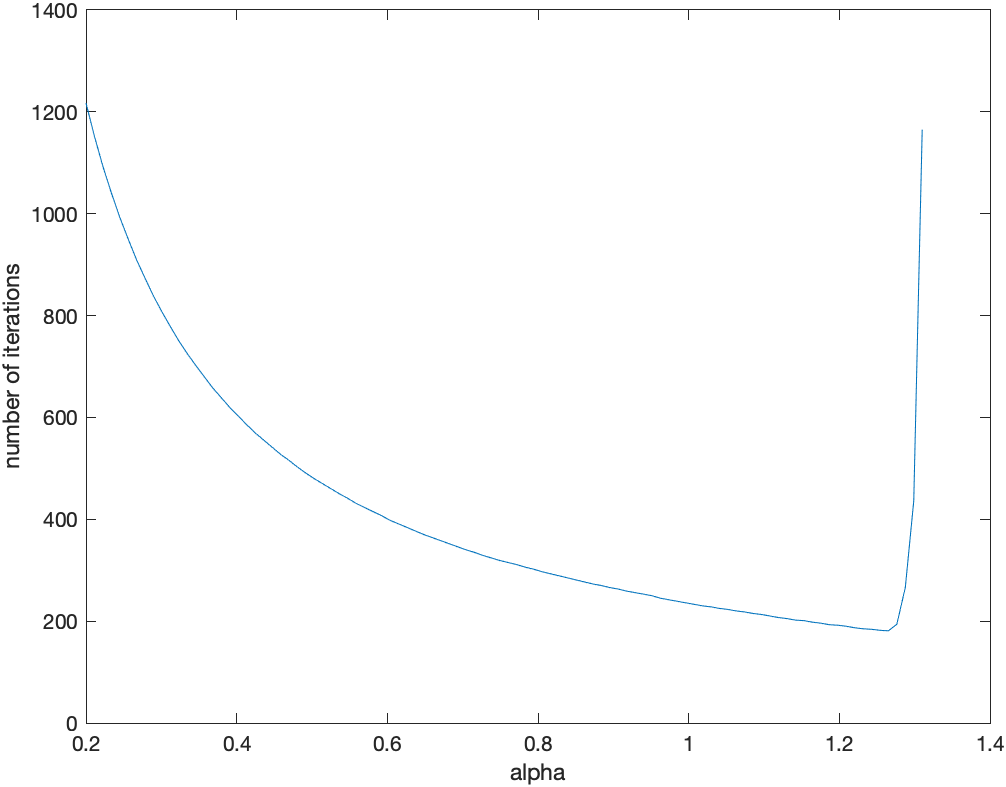
\includegraphics[width=.7\linewidth]{figs/Q2_iteration_alpha.png}
	\caption{The number of iterations needed to achieve $ ||\nabla f||<1e-6 $ for various $ \alpha $. Observe how the number of iterations first drop gently and then increase abruptly. $ \alpha = 1.2652 $ needs 181 iterations, which is fastest. }
	\label{fig:Q2_iteration_alpha}
\end{figure}

\begin{figure} 
	\begin{subfigure}[b]{.5\linewidth}
		\centering\large 	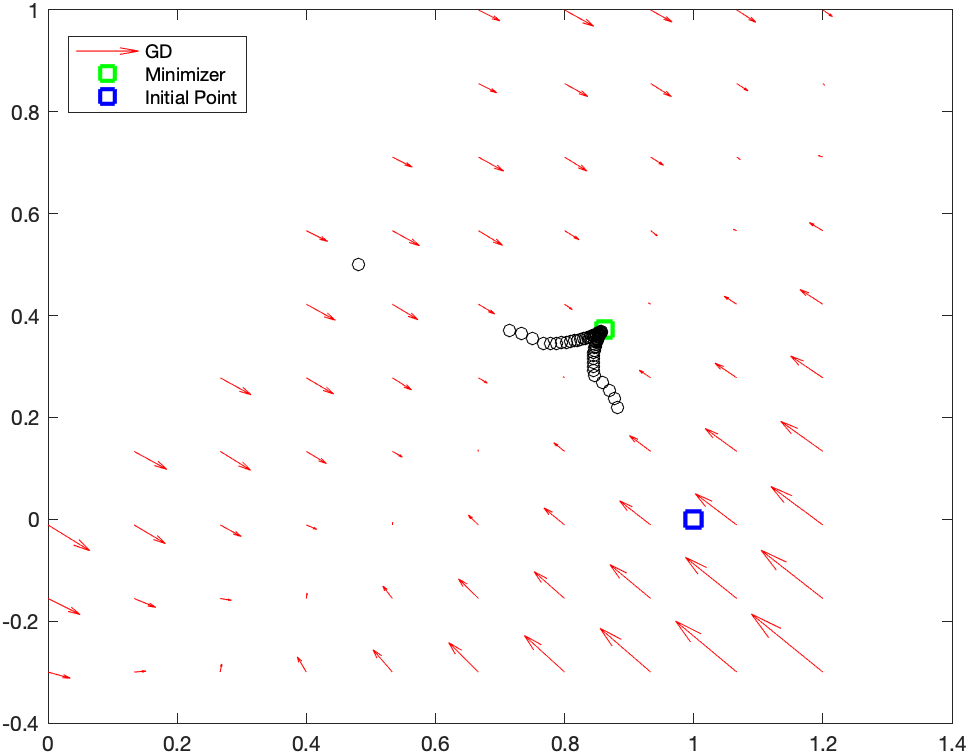
\includegraphics[width=\linewidth]{figs/Q2_12652}
		\caption{$ \alpha = 1.2652 $}
	\end{subfigure}% 
	\begin{subfigure}[b]{.515\linewidth}
		\centering\large 	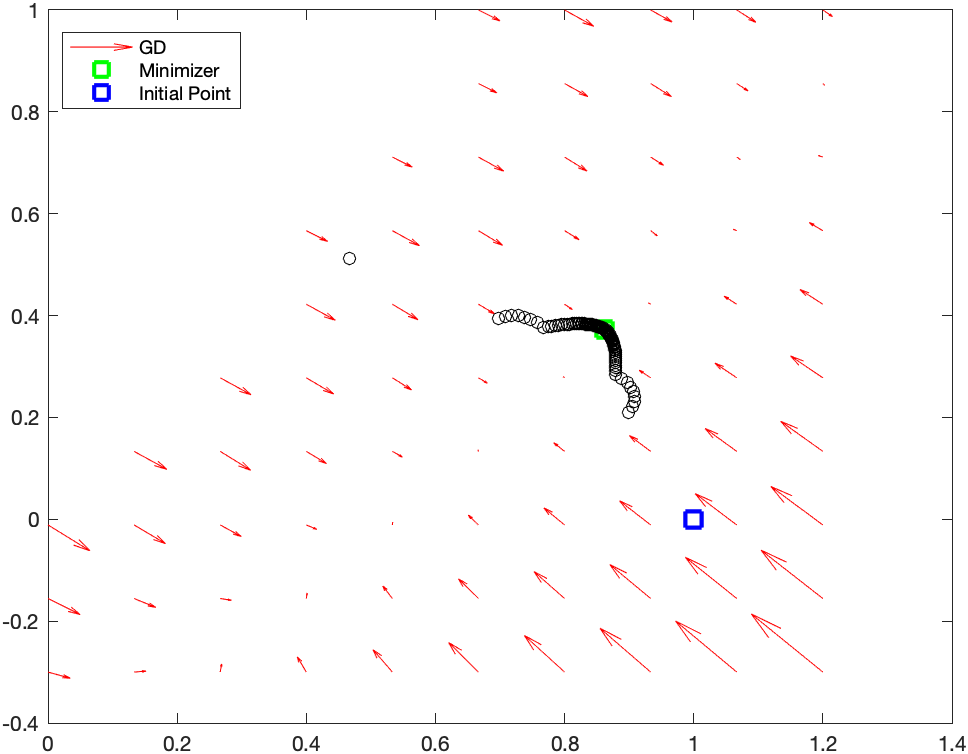
\includegraphics[width=\linewidth]{figs/Q2_12988}
		\caption{$ \alpha = 1.2988 $}
	\end{subfigure}
	\caption{The trajectories for the critical $ \alpha $ that results in an abrupt increase in the number of iterations needed for convergence. Observe that there is a \textbf{phase transition} in the geometry of the trajectories. Although oscillating behavior appears in both cases, notice that when $ \alpha = 1.2652 $, two oscillating curves converge in the same direction so there is not a lot waste in oscillating (and since $ \alpha = 1.2652 $ is large, convergence is fast). However, when $ \alpha = 1.2988 $, the two oscillating curves are converging in the opposite directions (so they are always oscillating to each other, wasteful!), which explains the sudden drop in the convergence speed.}\label{fig: Q2_increase}
\end{figure}

\section*{Q3: Stochastic Gradient Descent}
In this question, I use SGD with batch size 1 and I would like to find a strategy for stepsize reduction such that SGD will converge to the global minimizer. To this end, I decide to use the stepsize scheme where the stepsize at iteration $ k $ is given by $ \alpha_k = \alpha_0 \frac{M}{M+k} $, where $ \alpha_0 $ and $ M $ are tuning parameters. When $ \alpha_0 $ is fixed, larger $ M $ means slower decay of the stepsize. Recall that in class we have the convergence theory of SGD that, informally, if $ \alpha_0 $ is small enough (depending on the objective function $ f $),  an appropriate stepsize reduction scheme is used (an appropriate $ M $ in our case) and $ f $ satisfies some regularity conditions (such as convexity; not necessarily hold here), then SGD converges in expectation. In the following I will empirically look into different strategies. A good strategy should satisfy (a) convergence in expectation (b) converge with high probability (most trajectories converge) (c) fast convergence (d)  small error.


I found that $ M = 1000 $ performs well, so I tune $ \alpha_0 $, the initial stepsize. The average absolute error (with respect to $ x^{*} $) versus iteration is shown in Figure \ref{fig: Q3_iteration}, which can be used to verify whether SGD converge in expectation. It turns out that SGD converges (in expectation) when $ \alpha \leq 3 $. Interestingly, (deterministic) gradient descent will diverge with $ \alpha_0 = 3 $ as shown previously, even with the same stepsize reduction strategy (since it is messed up at the first step). Another observation is that, when $ \alpha_0 \leq 2 $, there is a "double descent" phenomenon where the error first drop at the very beginning, then increase and finally decrease again. When $ \alpha_0 <1 $, the first decrease will arrive at an error even smaller than the final error (the error at a reasonably large iteration). Lastly, when $ \alpha_0 > 4.65 $, SGD fails to converge. This is further verified in Figure \ref{fig: Q3_histogram}, where there is a small fraction of trajectories that does not converge when $ \alpha_0 = 4 $, and a large fraction when $ \alpha_0 = 4.65 $.

\begin{figure}[htp]
	
	\begin{subfigure}{.5\textwidth}
		\centering
		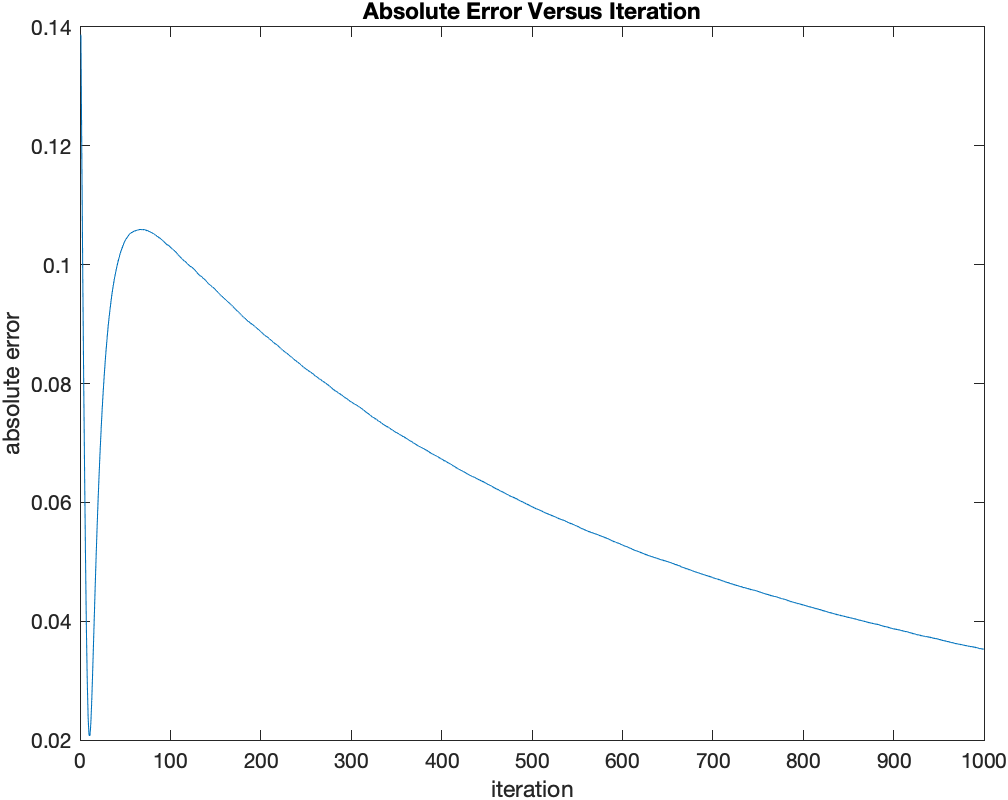
\includegraphics[width=0.9\linewidth]{figs/Q3/Iteration/M1000_a03.png}
		\caption{$ \alpha_0 = 0.3 $}
	\end{subfigure}
	\begin{subfigure}{.5\textwidth}
		\centering
		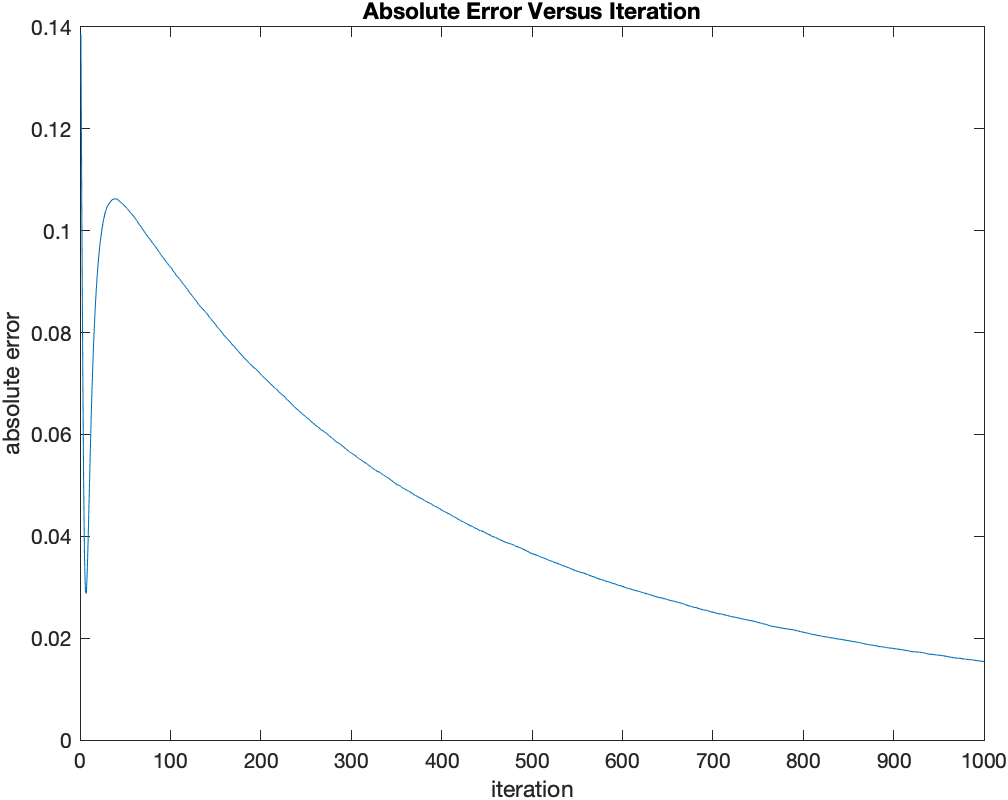
\includegraphics[width=0.9\linewidth]{figs/Q3/Iteration/M1000_a06.png}
		\caption{$ \alpha_0 = 0.6 $}
	\end{subfigure}
	\begin{subfigure}{.5\textwidth}
		\centering
		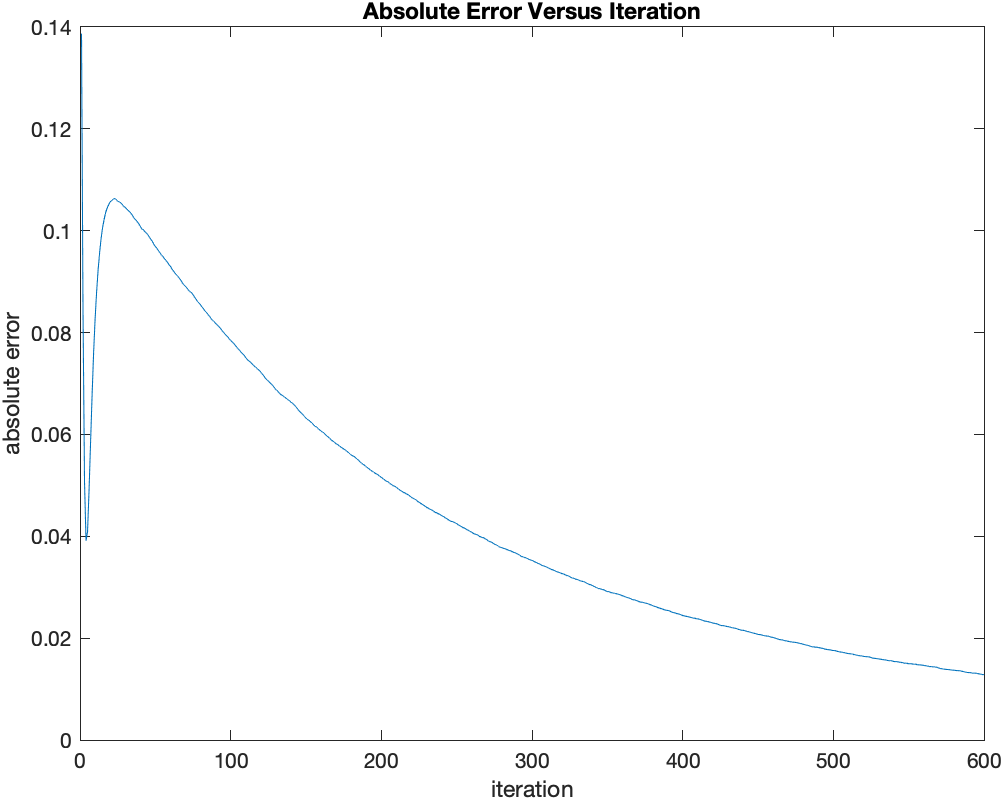
\includegraphics[width=0.9\linewidth]{figs/Q3/Iteration/M1000_a08.png}
		\caption{$ \alpha_0 = 0.8 $}
	\end{subfigure}
	\begin{subfigure}{.5\textwidth}
		\centering
		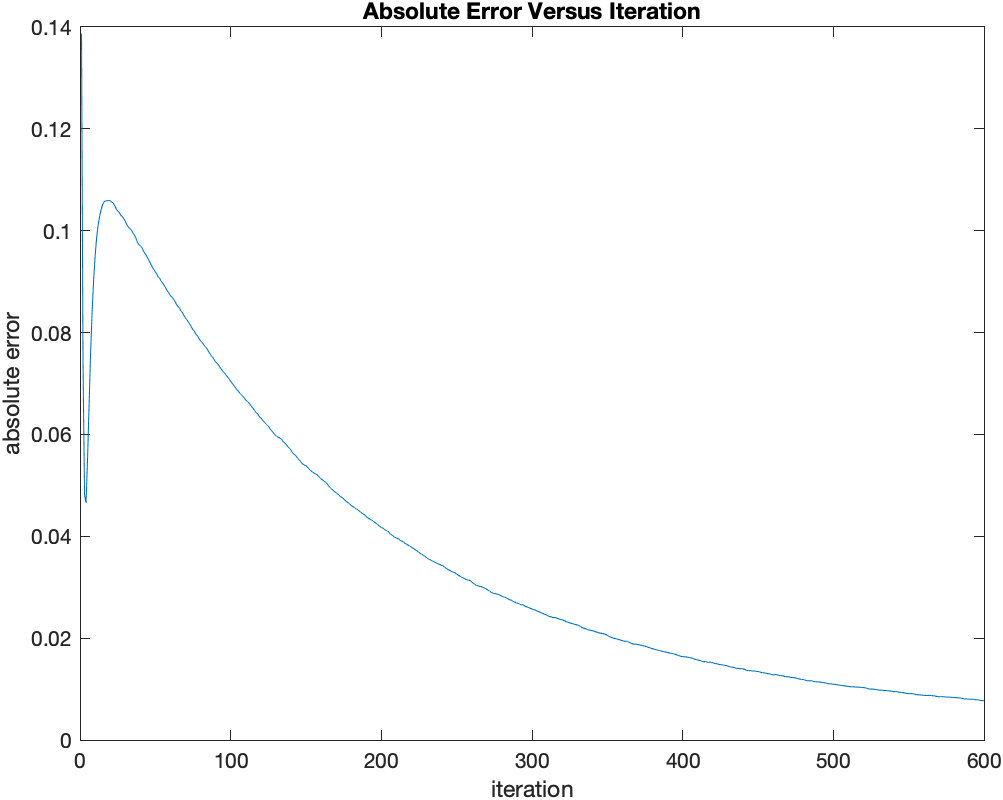
\includegraphics[width=0.9\linewidth]{figs/Q3/Iteration/M1000_a1.png}
		\caption{$ \alpha_0 = 1 $}
	\end{subfigure}
	\begin{subfigure}{.5\textwidth}
		\centering
		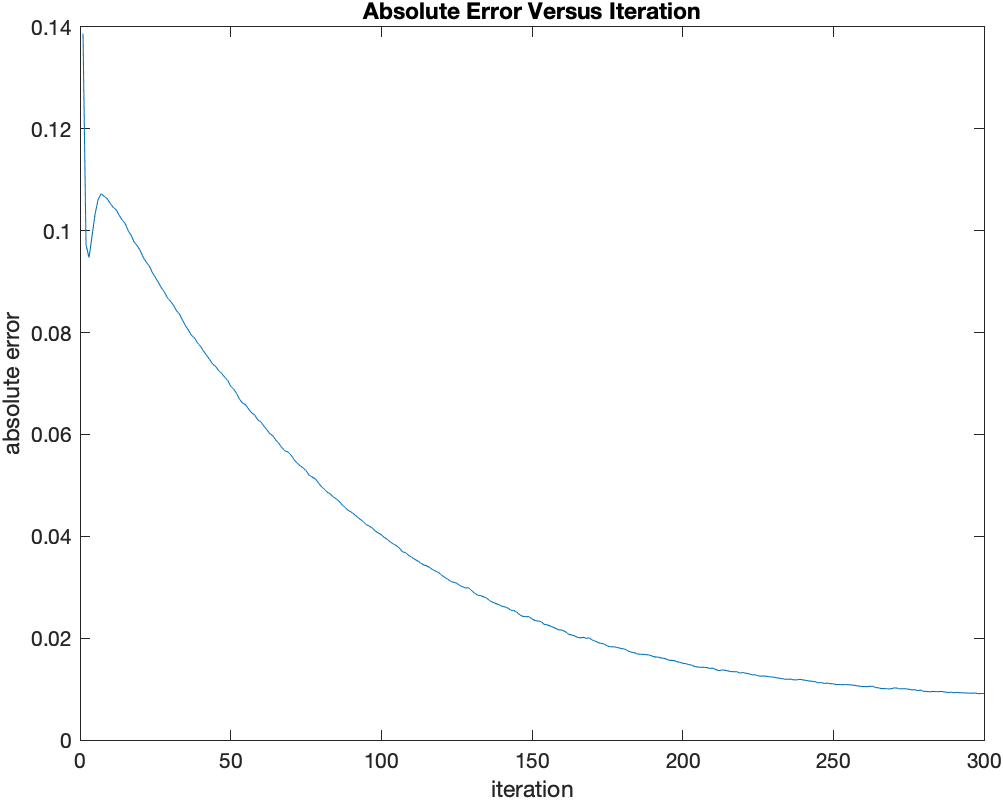
\includegraphics[width=0.9\linewidth]{figs/Q3/Iteration/M1000_a2.png}
		\caption{$ \alpha_0 = 2 $}
	\end{subfigure}
	\begin{subfigure}{.5\textwidth}
		\centering
		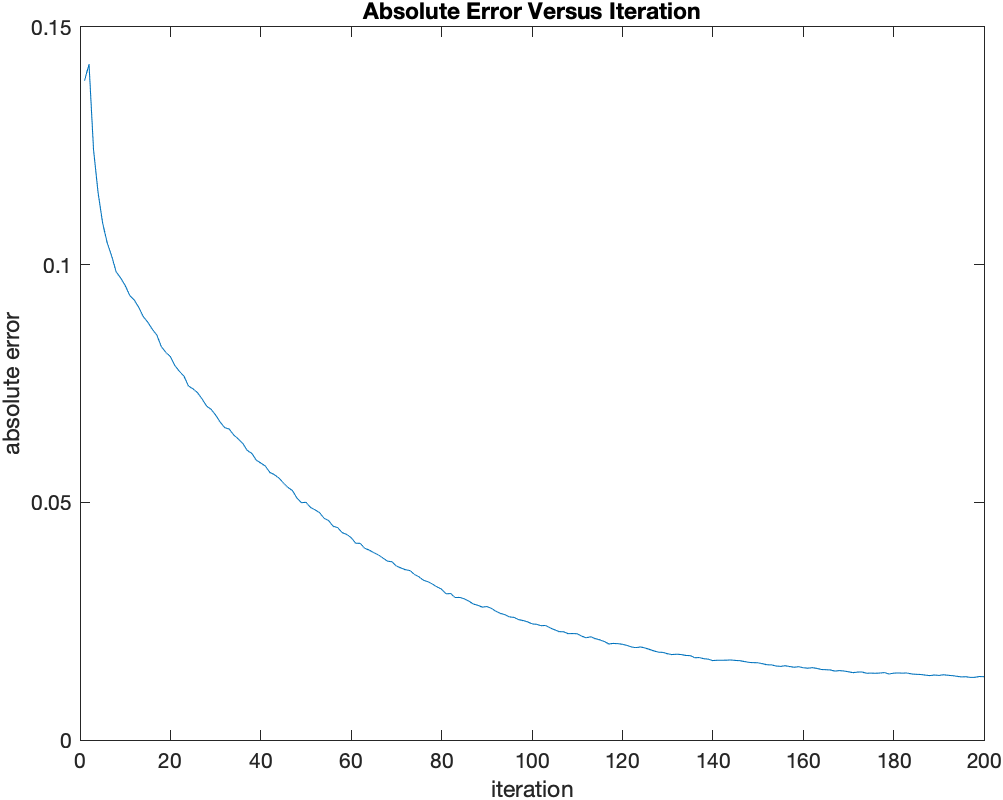
\includegraphics[width=0.9\linewidth]{figs/Q3/Iteration/M1000_a3.png}
		\caption{$ \alpha_0 = 3 $}
	\end{subfigure}
\begin{subfigure}{.5\textwidth}
	\centering
	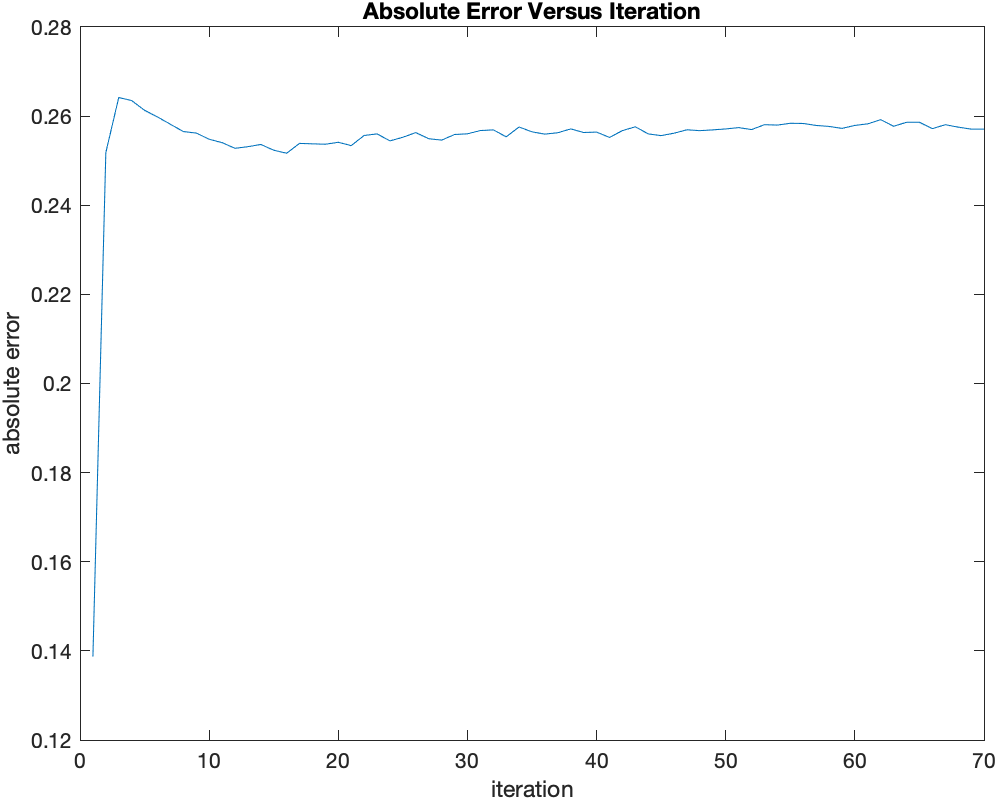
\includegraphics[width=0.9\linewidth]{figs/Q3/Iteration/M1000_a465.png}
	\caption{$ \alpha_0 = 4.65 $}
\end{subfigure}
\begin{subfigure}{.5\textwidth}
	\centering
	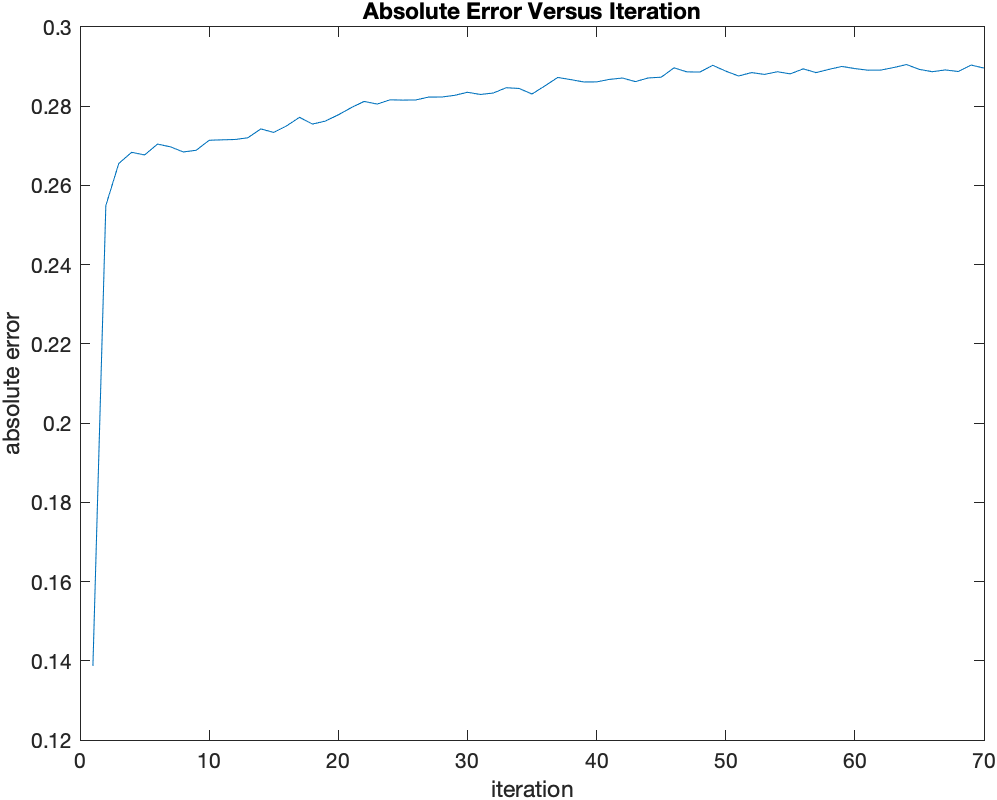
\includegraphics[width=0.9\linewidth]{figs/Q3/Iteration/M1000_a470.png}
	\caption{$ \alpha_0 = 4.70 $}
\end{subfigure}
	
	\caption{Absolute error (with respect to the global minimizer $ x^{\ast} $) versus iterations, when $ M = 1000 $. "Double descent" occurs when $ \alpha \leq 2 $. The plot is averaged over 1000 trajectories.}
	\label{fig: Q3_iteration}
	
\end{figure}


\begin{figure}[htp]
	
	\begin{subfigure}{.5\textwidth}
		\centering
		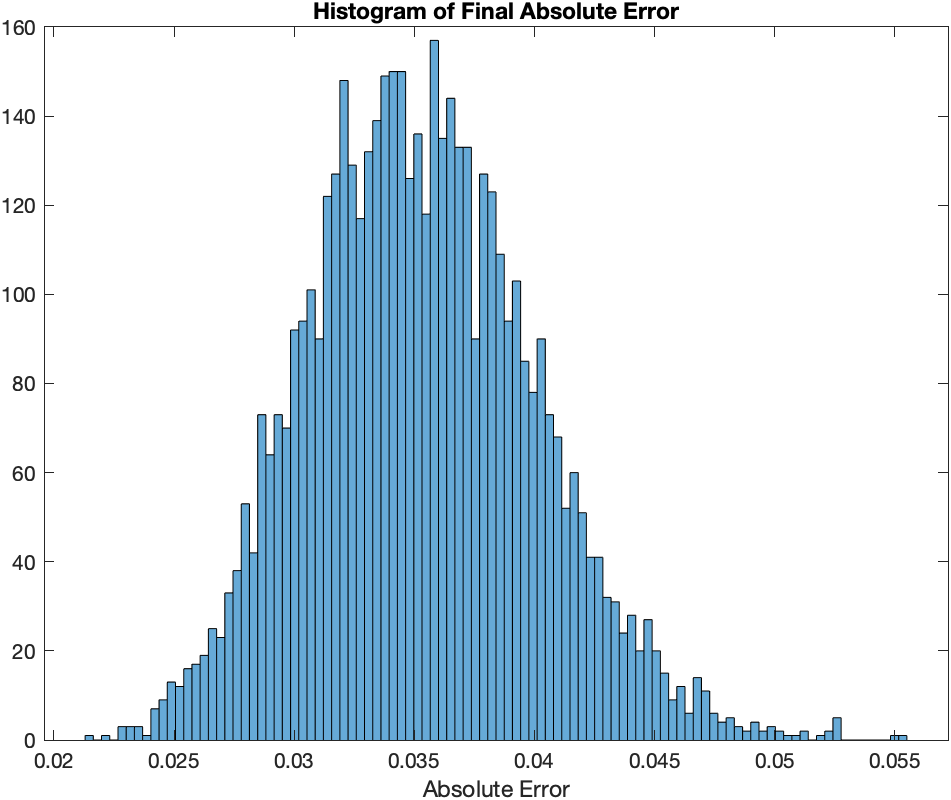
\includegraphics[width=0.8\linewidth]{figs/Q3/Histogram/M1000_a03.png}
		\caption{$ \alpha_0 = 0.3 $}
	\end{subfigure}
	\begin{subfigure}{.5\textwidth}
		\centering
		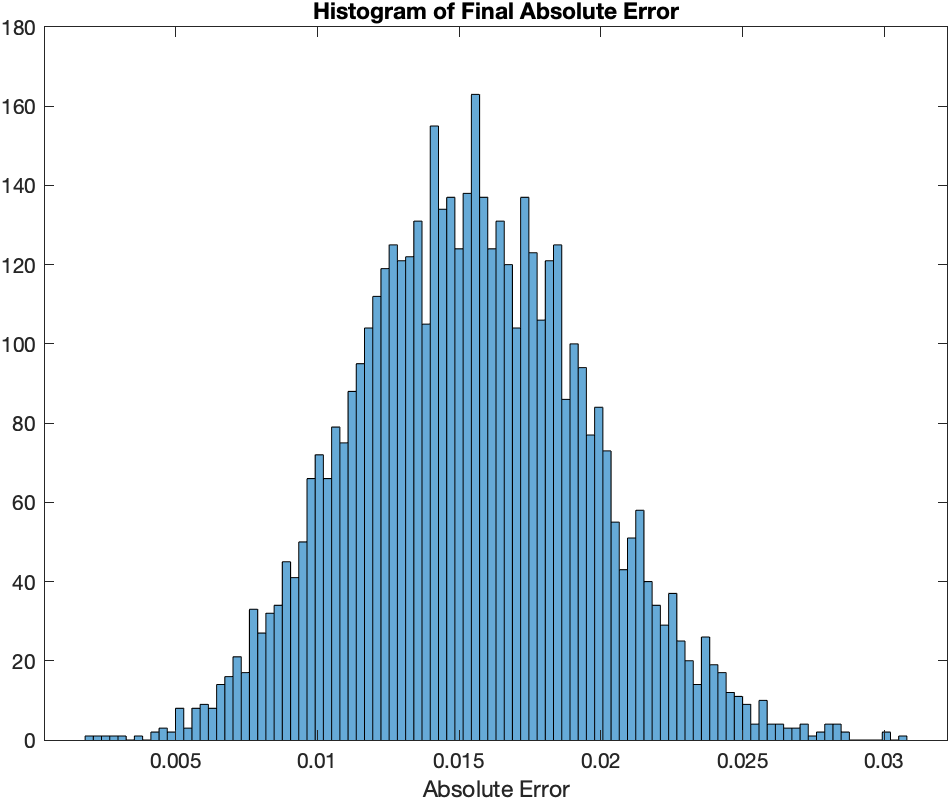
\includegraphics[width=0.8\linewidth]{figs/Q3/Histogram/M1000_a06.png}
		\caption{$ \alpha_0 = 0.6 $}
	\end{subfigure}
	\begin{subfigure}{.5\textwidth}
		\centering
		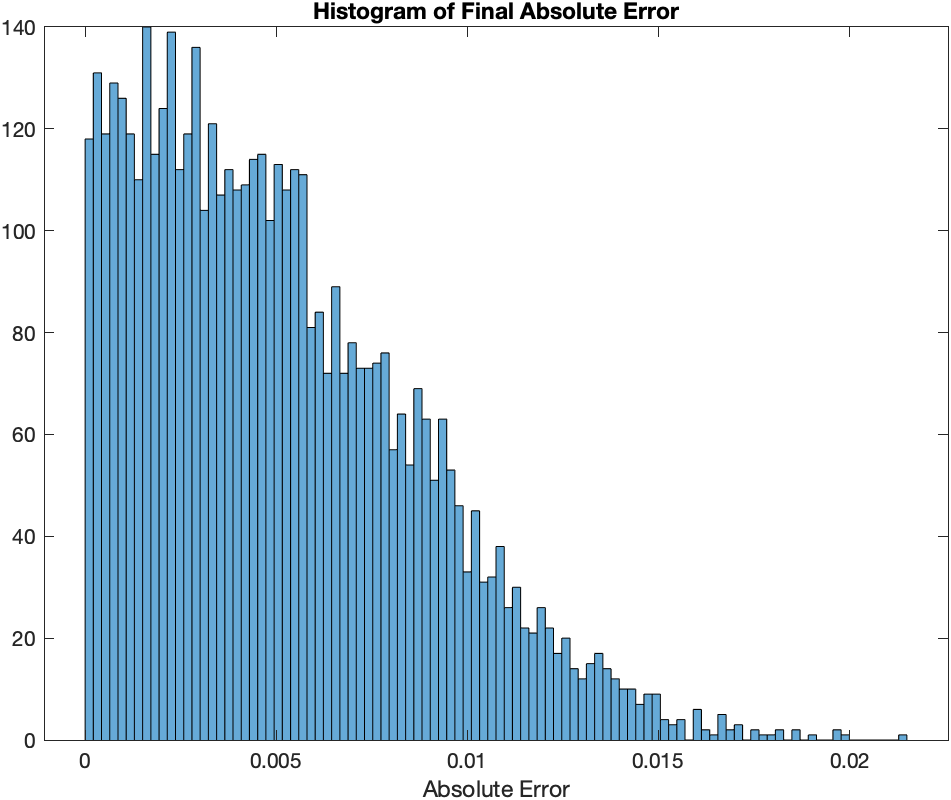
\includegraphics[width=0.8\linewidth]{figs/Q3/Histogram/M1000_a08.png}
		\caption{$ \alpha_0 = 0.8 $}
	\end{subfigure}
	\begin{subfigure}{.5\textwidth}
		\centering
		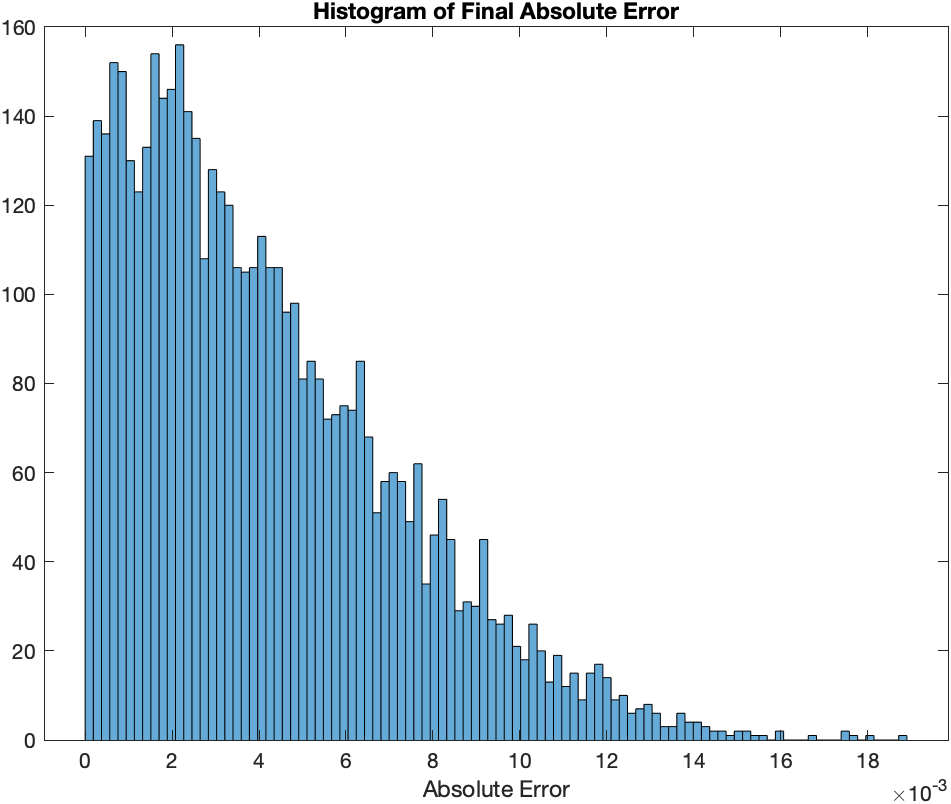
\includegraphics[width=0.8\linewidth]{figs/Q3/Histogram/M1000_a1.png}
		\caption{$ \alpha_0 = 1 $}
	\end{subfigure}
	\begin{subfigure}{.5\textwidth}
		\centering
		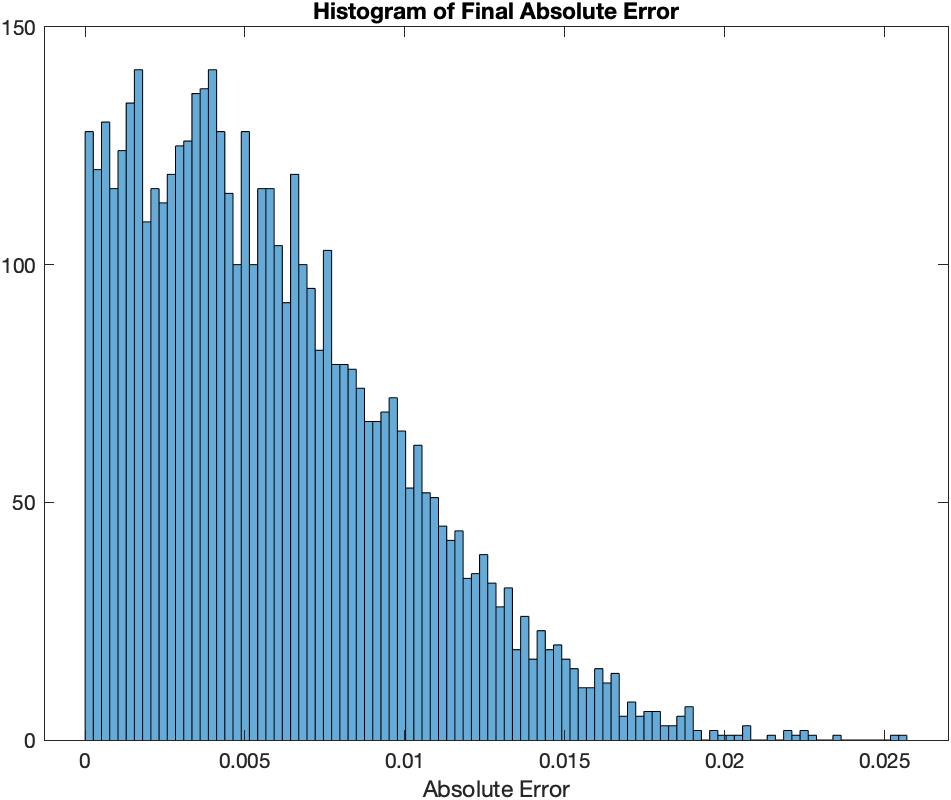
\includegraphics[width=0.8\linewidth]{figs/Q3/Histogram/M1000_a2.png}
		\caption{$ \alpha_0 = 2 $}
	\end{subfigure}
	\begin{subfigure}{.5\textwidth}
		\centering
		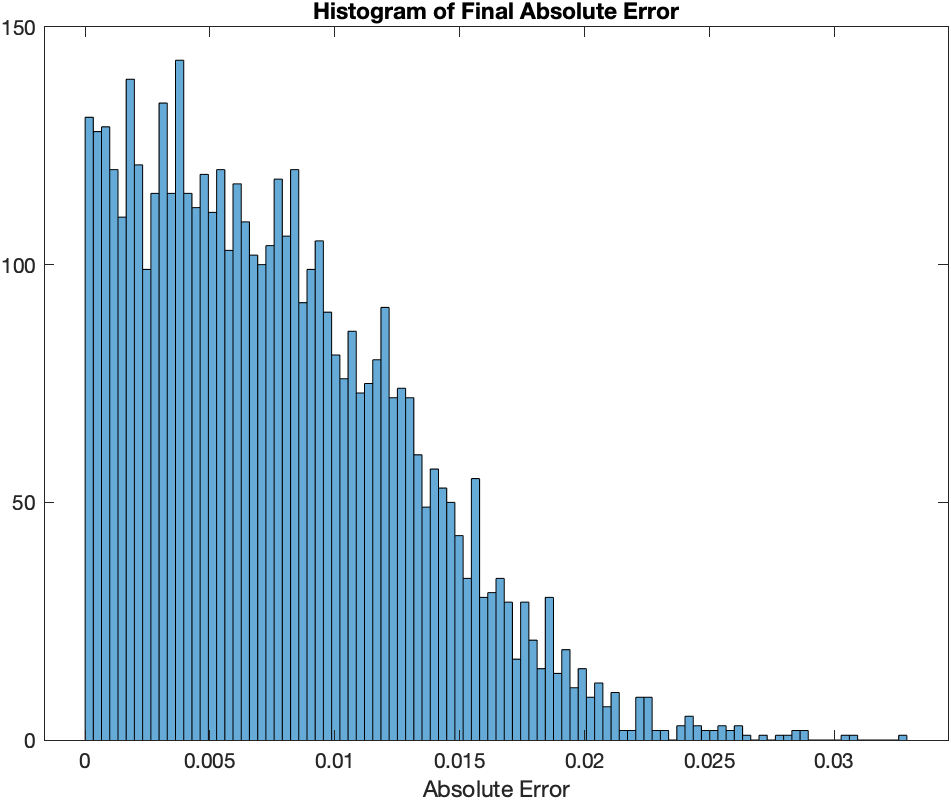
\includegraphics[width=0.8\linewidth]{figs/Q3/Histogram/M1000_a3.png}
		\caption{$ \alpha_0 = 3 $}
	\end{subfigure}
	\begin{subfigure}{.5\textwidth}
		\centering
		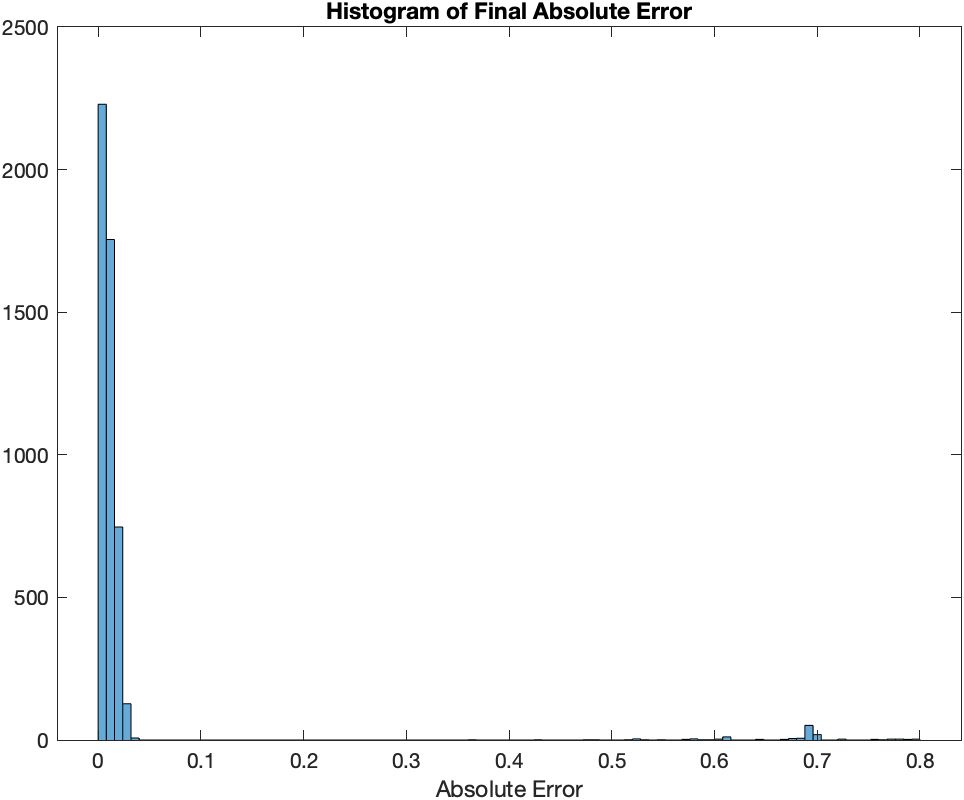
\includegraphics[width=0.8\linewidth]{figs/Q3/Histogram/M1000_a4.png}
		\caption{$ \alpha_0 = 4 $}
	\end{subfigure}
	\begin{subfigure}{.5\textwidth}
		\centering
		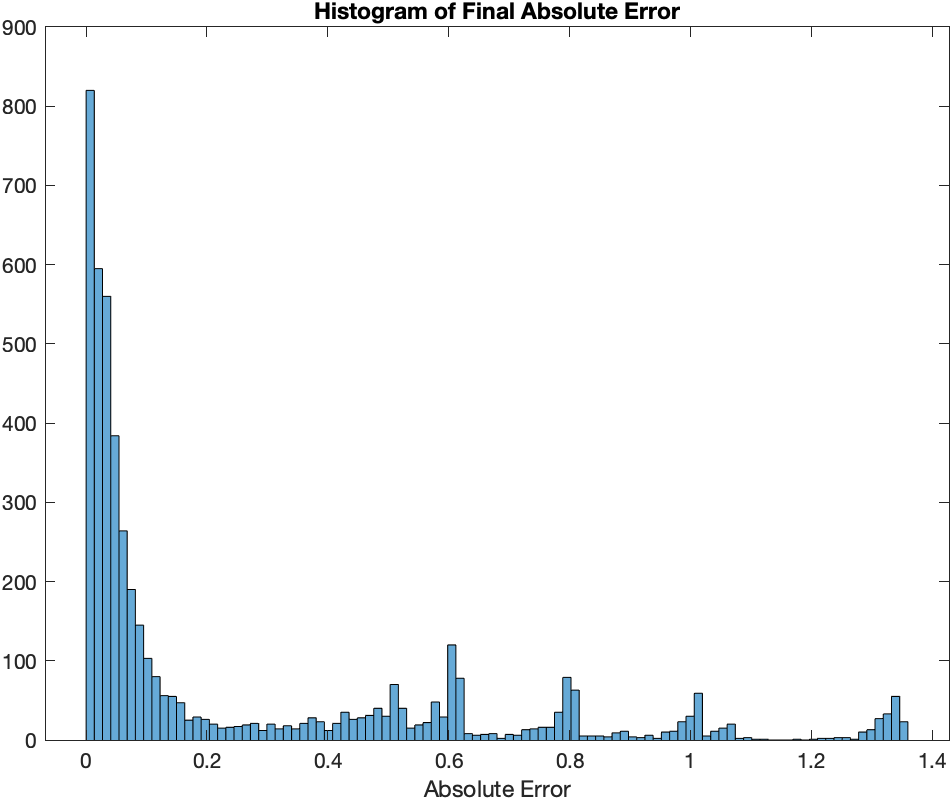
\includegraphics[width=0.8\linewidth]{figs/Q3/Histogram/M1000_a465.png}
		\caption{$ \alpha_0 = 4.65 $}
	\end{subfigure}
	
	\caption{Histogram of absolute error (with respect to the global minimizer $ x^{\ast} $), when $ M = 1000 $.  The plot is averaged over 1000 trajectories. When $ \alpha_0 = 4.65 $, there is relatively high probability that SGD will not converge to $ x^{*} $.}
	\label{fig: Q3_histogram}
	
\end{figure}

\paragraph{Which strategy should be used?} I find that $ \alpha_0 =2 $ should be used (that is, $ \alpha_k =2 \frac{1000}{1000+k} $). This is obtained by carefully observe Figure \ref{fig: Q3_iteration} and choose the one with fastest convergence and lowest error. Also, in Figure \ref{fig: Q3_histogram} we can see that with almost probability 1, the iterates converge to $ x^{*} $. This choice is further justified in Figure \ref{fig: Q3_choose_alpha}, where it is observed that the iterates tend to be stuck at a flat region (with small derivatives) and thus larger stepsize helps speed up convergence.

\paragraph{GD works better than SGD in the problem} Finally, note that since this is only a two-dimensional problem with only 6 data points, using SGD doesn't really contribute to computational efficiency. Also, GD converges faster and much closer to $ x^{*} $ than SGD: when $ \alpha_0 =1 $ with no stepsize reduction, GD achieves absolute error of 0.0027 with 100 iterations, while SGD (with stepsize reduction) gets an error of 0.01 with 600 iterations. 

\begin{figure} 
	\begin{subfigure}[b]{.5\linewidth}
		\centering\large 	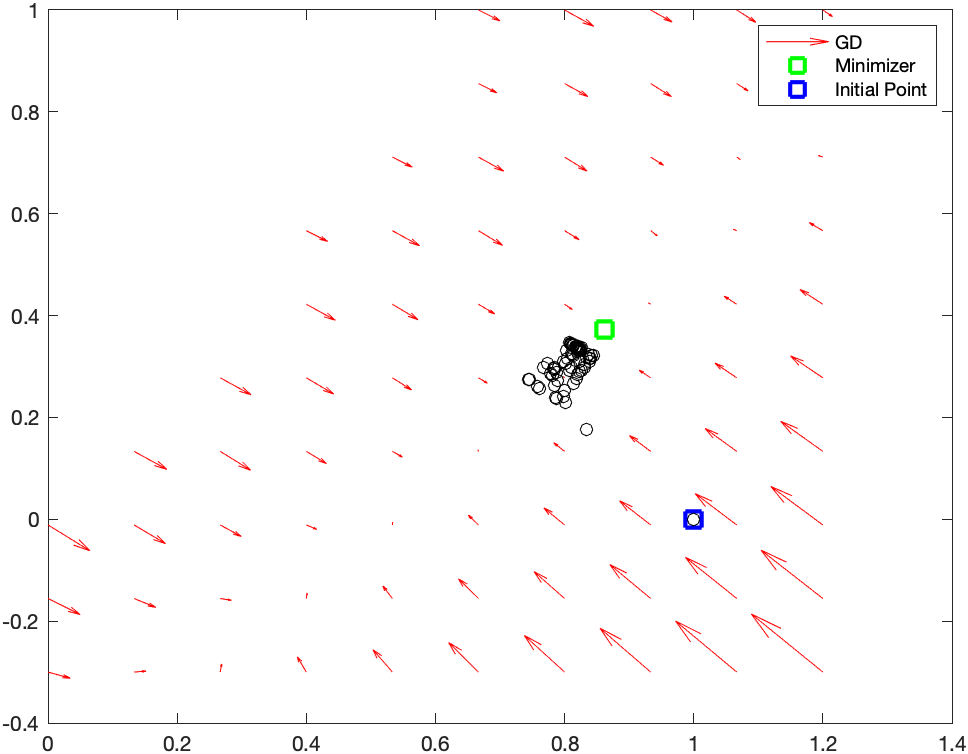
\includegraphics[width=\linewidth]{figs/Q3/a2_traj}
		\caption{$ \alpha_0 = 2 $}
	\end{subfigure}% 
	\begin{subfigure}[b]{.515\linewidth}
		\centering\large 	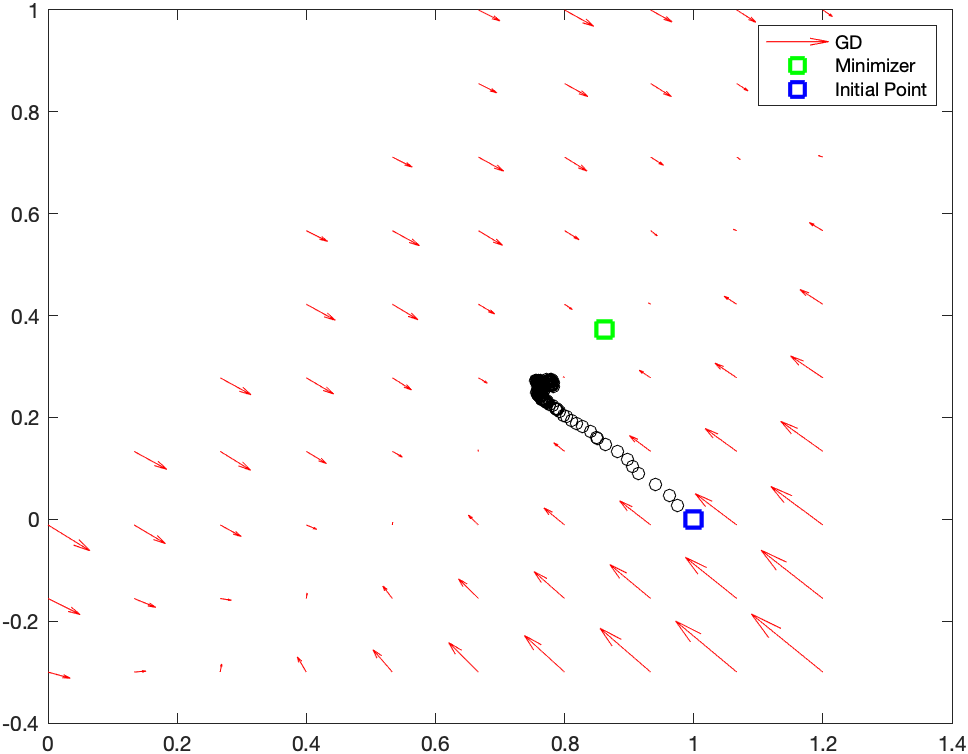
\includegraphics[width=\linewidth]{figs/Q3/a03_traj}
		\caption{$ \alpha_0 = 0.3 $}
	\end{subfigure}
	\caption{One trajectory for SGD. When $ \alpha_0 = 0.3 $, the iterates are stuck in the region where the gradient is small and therefore progress extremely slowly. Using larger stepsize such as $ \alpha_0 =2$ speeds up convergence significantly.}\label{fig: Q3_choose_alpha}
\end{figure}

\end{document}

				